\chapter{More about Types}
\label{ch:more-types}

So far we have learned about a few basic types (for example \isa{bool} and
\isa{nat}), type abbreviations (\isacommand{types}) and recursive datatypes
(\isacommand{datatype}). This chapter will introduce more
advanced material:
\begin{itemize}
\item Pairs ({\S}\ref{sec:products}) and records ({\S}\ref{sec:records}),
and how to reason about them.
\item Type classes: how to specify and reason about axiomatic collections of
  types ({\S}\ref{sec:axclass}). This section leads on to a discussion of
  Isabelle's numeric types ({\S}\ref{sec:numbers}).  
\item Introducing your own types: how to define types that
  cannot be constructed with any of the basic methods
  ({\S}\ref{sec:adv-typedef}).
\end{itemize}

The material in this section goes beyond the needs of most novices.
Serious users should at least skim the sections as far as type classes.
That material is fairly advanced; read the beginning to understand what it
is about, but consult the rest only when necessary.

\index{pairs and tuples|(}
%
\begin{isabellebody}%
\def\isabellecontext{Pairs}%
%
\isadelimtheory
%
\endisadelimtheory
%
\isatagtheory
%
\endisatagtheory
{\isafoldtheory}%
%
\isadelimtheory
%
\endisadelimtheory
%
\isamarkupsection{Pairs and Tuples%
}
\isamarkuptrue%
%
\begin{isamarkuptext}%
\label{sec:products}
Ordered pairs were already introduced in \S\ref{sec:pairs}, but only with a minimal
repertoire of operations: pairing and the two projections \isa{fst} and
\isa{snd}. In any non-trivial application of pairs you will find that this
quickly leads to unreadable nests of projections. This
section introduces syntactic sugar to overcome this
problem: pattern matching with tuples.%
\end{isamarkuptext}%
\isamarkuptrue%
%
\isamarkupsubsection{Pattern Matching with Tuples%
}
\isamarkuptrue%
%
\begin{isamarkuptext}%
Tuples may be used as patterns in $\lambda$-abstractions,
for example \isa{{\isasymlambda}{\isacharparenleft}x{\isacharcomma}y{\isacharcomma}z{\isacharparenright}{\isachardot}x{\isacharplus}y{\isacharplus}z} and \isa{{\isasymlambda}{\isacharparenleft}{\isacharparenleft}x{\isacharcomma}y{\isacharparenright}{\isacharcomma}z{\isacharparenright}{\isachardot}x{\isacharplus}y{\isacharplus}z}. In fact,
tuple patterns can be used in most variable binding constructs,
and they can be nested. Here are
some typical examples:
\begin{quote}
\isa{let\ {\isacharparenleft}x{\isacharcomma}\ y{\isacharparenright}\ {\isacharequal}\ f\ z\ in\ {\isacharparenleft}y{\isacharcomma}\ x{\isacharparenright}}\\
\isa{case\ xs\ of\ {\isacharbrackleft}{\isacharbrackright}\ {\isasymRightarrow}\ {\isadigit{0}}\ {\isacharbar}\ {\isacharparenleft}x{\isacharcomma}\ y{\isacharparenright}\ {\isacharhash}\ zs\ {\isasymRightarrow}\ x\ {\isacharplus}\ y}\\
\isa{{\isasymforall}{\isacharparenleft}x{\isacharcomma}y{\isacharparenright}{\isasymin}A{\isachardot}\ x{\isacharequal}y}\\
\isa{{\isacharbraceleft}{\isacharparenleft}x{\isacharcomma}y{\isacharcomma}z{\isacharparenright}{\isachardot}\ x{\isacharequal}z{\isacharbraceright}}\\
\isa{{\isasymUnion}\isactrlbsub {\isacharparenleft}x{\isacharcomma}\ y{\isacharparenright}{\isasymin}A\isactrlesub \ {\isacharbraceleft}x\ {\isacharplus}\ y{\isacharbraceright}}
\end{quote}
The intuitive meanings of these expressions should be obvious.
Unfortunately, we need to know in more detail what the notation really stands
for once we have to reason about it.  Abstraction
over pairs and tuples is merely a convenient shorthand for a more complex
internal representation.  Thus the internal and external form of a term may
differ, which can affect proofs. If you want to avoid this complication,
stick to \isa{fst} and \isa{snd} and write \isa{{\isasymlambda}p{\isachardot}\ fst\ p\ {\isacharplus}\ snd\ p}
instead of \isa{{\isasymlambda}{\isacharparenleft}x{\isacharcomma}y{\isacharparenright}{\isachardot}\ x{\isacharplus}y}.  These terms are distinct even though they
denote the same function.

Internally, \isa{{\isasymlambda}{\isacharparenleft}x{\isacharcomma}\ y{\isacharparenright}{\isachardot}\ t} becomes \isa{split\ {\isacharparenleft}{\isasymlambda}x\ y{\isachardot}\ t{\isacharparenright}}, where
\cdx{split} is the uncurrying function of type \isa{{\isacharparenleft}{\isacharprime}a\ {\isasymRightarrow}\ {\isacharprime}b\ {\isasymRightarrow}\ {\isacharprime}c{\isacharparenright}\ {\isasymRightarrow}\ {\isacharprime}a\ {\isasymtimes}\ {\isacharprime}b\ {\isasymRightarrow}\ {\isacharprime}c} defined as
\begin{center}
\isa{split\ {\isasymequiv}\ {\isasymlambda}c\ p{\isachardot}\ c\ {\isacharparenleft}fst\ p{\isacharparenright}\ {\isacharparenleft}snd\ p{\isacharparenright}}
\hfill(\isa{split{\isacharunderscore}def})
\end{center}
Pattern matching in
other variable binding constructs is translated similarly. Thus we need to
understand how to reason about such constructs.%
\end{isamarkuptext}%
\isamarkuptrue%
%
\isamarkupsubsection{Theorem Proving%
}
\isamarkuptrue%
%
\begin{isamarkuptext}%
The most obvious approach is the brute force expansion of \isa{split}:%
\end{isamarkuptext}%
\isamarkuptrue%
\isacommand{lemma}\isamarkupfalse%
\ {\isachardoublequoteopen}{\isacharparenleft}{\isasymlambda}{\isacharparenleft}x{\isacharcomma}y{\isacharparenright}{\isachardot}x{\isacharparenright}\ p\ {\isacharequal}\ fst\ p{\isachardoublequoteclose}\isanewline
%
\isadelimproof
%
\endisadelimproof
%
\isatagproof
\isacommand{by}\isamarkupfalse%
{\isacharparenleft}simp\ add{\isacharcolon}\ split{\isacharunderscore}def{\isacharparenright}%
\endisatagproof
{\isafoldproof}%
%
\isadelimproof
%
\endisadelimproof
%
\begin{isamarkuptext}%
This works well if rewriting with \isa{split{\isacharunderscore}def} finishes the
proof, as it does above.  But if it does not, you end up with exactly what
we are trying to avoid: nests of \isa{fst} and \isa{snd}. Thus this
approach is neither elegant nor very practical in large examples, although it
can be effective in small ones.

If we consider why this lemma presents a problem, 
we quickly realize that we need to replace the variable~\isa{p} by some pair \isa{{\isacharparenleft}a{\isacharcomma}\ b{\isacharparenright}}.  Then both sides of the
equation would simplify to \isa{a} by the simplification rules
\isa{split\ f\ {\isacharparenleft}a{\isacharcomma}\ b{\isacharparenright}\ {\isacharequal}\ f\ a\ b} and \isa{fst\ {\isacharparenleft}a{\isacharcomma}\ b{\isacharparenright}\ {\isacharequal}\ a}.  
To reason about tuple patterns requires some way of
converting a variable of product type into a pair.

In case of a subterm of the form \isa{split\ f\ p} this is easy: the split
rule \isa{split{\isacharunderscore}split} replaces \isa{p} by a pair:%
\index{*split (method)}%
\end{isamarkuptext}%
\isamarkuptrue%
\isacommand{lemma}\isamarkupfalse%
\ {\isachardoublequoteopen}{\isacharparenleft}{\isasymlambda}{\isacharparenleft}x{\isacharcomma}y{\isacharparenright}{\isachardot}y{\isacharparenright}\ p\ {\isacharequal}\ snd\ p{\isachardoublequoteclose}\isanewline
%
\isadelimproof
%
\endisadelimproof
%
\isatagproof
\isacommand{apply}\isamarkupfalse%
{\isacharparenleft}split\ split{\isacharunderscore}split{\isacharparenright}%
\begin{isamarkuptxt}%
\begin{isabelle}%
\ {\isadigit{1}}{\isachardot}\ {\isasymforall}x\ y{\isachardot}\ p\ {\isacharequal}\ {\isacharparenleft}x{\isacharcomma}\ y{\isacharparenright}\ {\isasymlongrightarrow}\ y\ {\isacharequal}\ snd\ p%
\end{isabelle}
This subgoal is easily proved by simplification. Thus we could have combined
simplification and splitting in one command that proves the goal outright:%
\end{isamarkuptxt}%
\isamarkuptrue%
%
\endisatagproof
{\isafoldproof}%
%
\isadelimproof
%
\endisadelimproof
%
\isadelimproof
%
\endisadelimproof
%
\isatagproof
\isacommand{by}\isamarkupfalse%
{\isacharparenleft}simp\ split{\isacharcolon}\ split{\isacharunderscore}split{\isacharparenright}%
\endisatagproof
{\isafoldproof}%
%
\isadelimproof
%
\endisadelimproof
%
\begin{isamarkuptext}%
Let us look at a second example:%
\end{isamarkuptext}%
\isamarkuptrue%
\isacommand{lemma}\isamarkupfalse%
\ {\isachardoublequoteopen}let\ {\isacharparenleft}x{\isacharcomma}y{\isacharparenright}\ {\isacharequal}\ p\ in\ fst\ p\ {\isacharequal}\ x{\isachardoublequoteclose}\isanewline
%
\isadelimproof
%
\endisadelimproof
%
\isatagproof
\isacommand{apply}\isamarkupfalse%
{\isacharparenleft}simp\ only{\isacharcolon}\ Let{\isacharunderscore}def{\isacharparenright}%
\begin{isamarkuptxt}%
\begin{isabelle}%
\ {\isadigit{1}}{\isachardot}\ {\isacharparenleft}{\isasymlambda}{\isacharparenleft}x{\isacharcomma}\ y{\isacharparenright}{\isachardot}\ fst\ p\ {\isacharequal}\ x{\isacharparenright}\ p%
\end{isabelle}
A paired \isa{let} reduces to a paired $\lambda$-abstraction, which
can be split as above. The same is true for paired set comprehension:%
\end{isamarkuptxt}%
\isamarkuptrue%
%
\endisatagproof
{\isafoldproof}%
%
\isadelimproof
%
\endisadelimproof
\isacommand{lemma}\isamarkupfalse%
\ {\isachardoublequoteopen}p\ {\isasymin}\ {\isacharbraceleft}{\isacharparenleft}x{\isacharcomma}y{\isacharparenright}{\isachardot}\ x{\isacharequal}y{\isacharbraceright}\ {\isasymlongrightarrow}\ fst\ p\ {\isacharequal}\ snd\ p{\isachardoublequoteclose}\isanewline
%
\isadelimproof
%
\endisadelimproof
%
\isatagproof
\isacommand{apply}\isamarkupfalse%
\ simp%
\begin{isamarkuptxt}%
\begin{isabelle}%
\ {\isadigit{1}}{\isachardot}\ split\ op\ {\isacharequal}\ p\ {\isasymlongrightarrow}\ fst\ p\ {\isacharequal}\ snd\ p%
\end{isabelle}
Again, simplification produces a term suitable for \isa{split{\isacharunderscore}split}
as above. If you are worried about the strange form of the premise:
\isa{{\isasymlambda}{\isacharparenleft}x{\isacharcomma}\ y{\isacharparenright}{\isachardot}\ x\ {\isacharequal}\ y} is short for \isa{{\isasymlambda}{\isacharparenleft}x{\isacharcomma}y{\isacharparenright}{\isachardot}\ x{\isacharequal}y}.
The same proof procedure works for%
\end{isamarkuptxt}%
\isamarkuptrue%
%
\endisatagproof
{\isafoldproof}%
%
\isadelimproof
%
\endisadelimproof
\isacommand{lemma}\isamarkupfalse%
\ {\isachardoublequoteopen}p\ {\isasymin}\ {\isacharbraceleft}{\isacharparenleft}x{\isacharcomma}y{\isacharparenright}{\isachardot}\ x{\isacharequal}y{\isacharbraceright}\ {\isasymLongrightarrow}\ fst\ p\ {\isacharequal}\ snd\ p{\isachardoublequoteclose}%
\isadelimproof
%
\endisadelimproof
%
\isatagproof
%
\begin{isamarkuptxt}%
\noindent
except that we now have to use \isa{split{\isacharunderscore}split{\isacharunderscore}asm}, because
\isa{split} occurs in the assumptions.

However, splitting \isa{split} is not always a solution, as no \isa{split}
may be present in the goal. Consider the following function:%
\end{isamarkuptxt}%
\isamarkuptrue%
%
\endisatagproof
{\isafoldproof}%
%
\isadelimproof
%
\endisadelimproof
\isacommand{consts}\isamarkupfalse%
\ swap\ {\isacharcolon}{\isacharcolon}\ {\isachardoublequoteopen}{\isacharprime}a\ {\isasymtimes}\ {\isacharprime}b\ {\isasymRightarrow}\ {\isacharprime}b\ {\isasymtimes}\ {\isacharprime}a{\isachardoublequoteclose}\isanewline
\isacommand{primrec}\isamarkupfalse%
\isanewline
\ \ {\isachardoublequoteopen}swap\ {\isacharparenleft}x{\isacharcomma}y{\isacharparenright}\ {\isacharequal}\ {\isacharparenleft}y{\isacharcomma}x{\isacharparenright}{\isachardoublequoteclose}%
\begin{isamarkuptext}%
\noindent
Note that the above \isacommand{primrec} definition is admissible
because \isa{{\isasymtimes}} is a datatype. When we now try to prove%
\end{isamarkuptext}%
\isamarkuptrue%
\isacommand{lemma}\isamarkupfalse%
\ {\isachardoublequoteopen}swap{\isacharparenleft}swap\ p{\isacharparenright}\ {\isacharequal}\ p{\isachardoublequoteclose}%
\isadelimproof
%
\endisadelimproof
%
\isatagproof
%
\begin{isamarkuptxt}%
\noindent
simplification will do nothing, because the defining equation for \isa{Pairs{\isachardot}swap}
expects a pair. Again, we need to turn \isa{p} into a pair first, but this
time there is no \isa{split} in sight. In this case the only thing we can do
is to split the term by hand:%
\end{isamarkuptxt}%
\isamarkuptrue%
\isacommand{apply}\isamarkupfalse%
{\isacharparenleft}case{\isacharunderscore}tac\ p{\isacharparenright}%
\begin{isamarkuptxt}%
\noindent
\begin{isabelle}%
\ {\isadigit{1}}{\isachardot}\ {\isasymAnd}a\ b{\isachardot}\ p\ {\isacharequal}\ {\isacharparenleft}a{\isacharcomma}\ b{\isacharparenright}\ {\isasymLongrightarrow}\ Pairs{\isachardot}swap\ {\isacharparenleft}Pairs{\isachardot}swap\ p{\isacharparenright}\ {\isacharequal}\ p%
\end{isabelle}
Again, \methdx{case_tac} is applicable because \isa{{\isasymtimes}} is a datatype.
The subgoal is easily proved by \isa{simp}.

Splitting by \isa{case{\isacharunderscore}tac} also solves the previous examples and may thus
appear preferable to the more arcane methods introduced first. However, see
the warning about \isa{case{\isacharunderscore}tac} in \S\ref{sec:struct-ind-case}.

In case the term to be split is a quantified variable, there are more options.
You can split \emph{all} \isa{{\isasymAnd}}-quantified variables in a goal
with the rewrite rule \isa{split{\isacharunderscore}paired{\isacharunderscore}all}:%
\end{isamarkuptxt}%
\isamarkuptrue%
%
\endisatagproof
{\isafoldproof}%
%
\isadelimproof
%
\endisadelimproof
\isacommand{lemma}\isamarkupfalse%
\ {\isachardoublequoteopen}{\isasymAnd}p\ q{\isachardot}\ swap{\isacharparenleft}swap\ p{\isacharparenright}\ {\isacharequal}\ q\ {\isasymlongrightarrow}\ p\ {\isacharequal}\ q{\isachardoublequoteclose}\isanewline
%
\isadelimproof
%
\endisadelimproof
%
\isatagproof
\isacommand{apply}\isamarkupfalse%
{\isacharparenleft}simp\ only{\isacharcolon}\ split{\isacharunderscore}paired{\isacharunderscore}all{\isacharparenright}%
\begin{isamarkuptxt}%
\noindent
\begin{isabelle}%
\ {\isadigit{1}}{\isachardot}\ {\isasymAnd}a\ b\ aa\ ba{\isachardot}\isanewline
\isaindent{\ {\isadigit{1}}{\isachardot}\ \ \ \ }Pairs{\isachardot}swap\ {\isacharparenleft}Pairs{\isachardot}swap\ {\isacharparenleft}a{\isacharcomma}\ b{\isacharparenright}{\isacharparenright}\ {\isacharequal}\ {\isacharparenleft}aa{\isacharcomma}\ ba{\isacharparenright}\ {\isasymlongrightarrow}\isanewline
\isaindent{\ {\isadigit{1}}{\isachardot}\ \ \ \ }{\isacharparenleft}a{\isacharcomma}\ b{\isacharparenright}\ {\isacharequal}\ {\isacharparenleft}aa{\isacharcomma}\ ba{\isacharparenright}%
\end{isabelle}%
\end{isamarkuptxt}%
\isamarkuptrue%
\isacommand{apply}\isamarkupfalse%
\ simp\isanewline
\isacommand{done}\isamarkupfalse%
%
\endisatagproof
{\isafoldproof}%
%
\isadelimproof
%
\endisadelimproof
%
\begin{isamarkuptext}%
\noindent
Note that we have intentionally included only \isa{split{\isacharunderscore}paired{\isacharunderscore}all}
in the first simplification step, and then we simplify again. 
This time the reason was not merely
pedagogical:
\isa{split{\isacharunderscore}paired{\isacharunderscore}all} may interfere with other functions
of the simplifier.
The following command could fail (here it does not)
where two separate \isa{simp} applications succeed.%
\end{isamarkuptext}%
\isamarkuptrue%
%
\isadelimproof
%
\endisadelimproof
%
\isatagproof
\isacommand{apply}\isamarkupfalse%
{\isacharparenleft}simp\ add{\isacharcolon}\ split{\isacharunderscore}paired{\isacharunderscore}all{\isacharparenright}%
\endisatagproof
{\isafoldproof}%
%
\isadelimproof
%
\endisadelimproof
%
\begin{isamarkuptext}%
\noindent
Finally, the simplifier automatically splits all \isa{{\isasymforall}} and
\isa{{\isasymexists}}-quantified variables:%
\end{isamarkuptext}%
\isamarkuptrue%
\isacommand{lemma}\isamarkupfalse%
\ {\isachardoublequoteopen}{\isasymforall}p{\isachardot}\ {\isasymexists}q{\isachardot}\ swap\ p\ {\isacharequal}\ swap\ q{\isachardoublequoteclose}\isanewline
%
\isadelimproof
%
\endisadelimproof
%
\isatagproof
\isacommand{by}\isamarkupfalse%
\ simp%
\endisatagproof
{\isafoldproof}%
%
\isadelimproof
%
\endisadelimproof
%
\begin{isamarkuptext}%
\noindent
To turn off this automatic splitting, just disable the
responsible simplification rules:
\begin{center}
\isa{{\isacharparenleft}{\isasymforall}x{\isachardot}\ P\ x{\isacharparenright}\ {\isacharequal}\ {\isacharparenleft}{\isasymforall}a\ b{\isachardot}\ P\ {\isacharparenleft}a{\isacharcomma}\ b{\isacharparenright}{\isacharparenright}}
\hfill
(\isa{split{\isacharunderscore}paired{\isacharunderscore}All})\\
\isa{{\isacharparenleft}{\isasymexists}x{\isachardot}\ P\ x{\isacharparenright}\ {\isacharequal}\ {\isacharparenleft}{\isasymexists}a\ b{\isachardot}\ P\ {\isacharparenleft}a{\isacharcomma}\ b{\isacharparenright}{\isacharparenright}}
\hfill
(\isa{split{\isacharunderscore}paired{\isacharunderscore}Ex})
\end{center}%
\end{isamarkuptext}%
\isamarkuptrue%
%
\isadelimtheory
%
\endisadelimtheory
%
\isatagtheory
%
\endisatagtheory
{\isafoldtheory}%
%
\isadelimtheory
%
\endisadelimtheory
\end{isabellebody}%
%%% Local Variables:
%%% mode: latex
%%% TeX-master: "root"
%%% End:
    %%%Section "Pairs and Tuples"
\index{pairs and tuples|)}

%
\begin{isabellebody}%
\def\isabellecontext{Records}%
%
\isamarkupheader{Records \label{sec:records}%
}
\isamarkuptrue%
%
\isadelimtheory
%
\endisadelimtheory
%
\isatagtheory
%
\endisatagtheory
{\isafoldtheory}%
%
\isadelimtheory
%
\endisadelimtheory
%
\begin{isamarkuptext}%
\index{records|(}%
  Records are familiar from programming languages.  A record of $n$
  fields is essentially an $n$-tuple, but the record's components have
  names, which can make expressions easier to read and reduces the
  risk of confusing one field for another.

  A record of Isabelle/HOL covers a collection of fields, with select
  and update operations.  Each field has a specified type, which may
  be polymorphic.  The field names are part of the record type, and
  the order of the fields is significant --- as it is in Pascal but
  not in Standard ML.  If two different record types have field names
  in common, then the ambiguity is resolved in the usual way, by
  qualified names.

  Record types can also be defined by extending other record types.
  Extensible records make use of the reserved pseudo-field \cdx{more},
  which is present in every record type.  Generic record operations
  work on all possible extensions of a given type scheme; polymorphism
  takes care of structural sub-typing behind the scenes.  There are
  also explicit coercion functions between fixed record types.%
\end{isamarkuptext}%
\isamarkuptrue%
%
\isamarkupsubsection{Record Basics%
}
\isamarkuptrue%
%
\begin{isamarkuptext}%
Record types are not primitive in Isabelle and have a delicate
  internal representation \cite{NaraschewskiW-TPHOLs98}, based on
  nested copies of the primitive product type.  A \commdx{record}
  declaration introduces a new record type scheme by specifying its
  fields, which are packaged internally to hold up the perception of
  the record as a distinguished entity.  Here is a simple example:%
\end{isamarkuptext}%
\isamarkuptrue%
\isacommand{record}\isamarkupfalse%
\ point\ {\isacharequal}\isanewline
\ \ Xcoord\ {\isacharcolon}{\isacharcolon}\ int\isanewline
\ \ Ycoord\ {\isacharcolon}{\isacharcolon}\ int%
\begin{isamarkuptext}%
Records of type \isa{point} have two fields named \isa{Xcoord}
  and \isa{Ycoord}, both of type~\isa{int}.  We now define a
  constant of type \isa{point}:%
\end{isamarkuptext}%
\isamarkuptrue%
\isacommand{constdefs}\isamarkupfalse%
\isanewline
\ \ pt{\isadigit{1}}\ {\isacharcolon}{\isacharcolon}\ point\isanewline
\ \ {\isachardoublequoteopen}pt{\isadigit{1}}\ {\isasymequiv}\ {\isacharparenleft}{\isacharbar}\ Xcoord\ {\isacharequal}\ {\isadigit{9}}{\isadigit{9}}{\isadigit{9}}{\isacharcomma}\ Ycoord\ {\isacharequal}\ {\isadigit{2}}{\isadigit{3}}\ {\isacharbar}{\isacharparenright}{\isachardoublequoteclose}%
\begin{isamarkuptext}%
We see above the ASCII notation for record brackets.  You can also
  use the symbolic brackets \isa{{\isasymlparr}} and \isa{{\isasymrparr}}.  Record type
  expressions can be also written directly with individual fields.
  The type name above is merely an abbreviation.%
\end{isamarkuptext}%
\isamarkuptrue%
\isacommand{constdefs}\isamarkupfalse%
\isanewline
\ \ pt{\isadigit{2}}\ {\isacharcolon}{\isacharcolon}\ {\isachardoublequoteopen}{\isasymlparr}Xcoord\ {\isacharcolon}{\isacharcolon}\ int{\isacharcomma}\ Ycoord\ {\isacharcolon}{\isacharcolon}\ int{\isasymrparr}{\isachardoublequoteclose}\isanewline
\ \ {\isachardoublequoteopen}pt{\isadigit{2}}\ {\isasymequiv}\ {\isasymlparr}Xcoord\ {\isacharequal}\ {\isacharminus}{\isadigit{4}}{\isadigit{5}}{\isacharcomma}\ Ycoord\ {\isacharequal}\ {\isadigit{9}}{\isadigit{7}}{\isasymrparr}{\isachardoublequoteclose}%
\begin{isamarkuptext}%
For each field, there is a \emph{selector}\index{selector!record}
  function of the same name.  For example, if \isa{p} has type \isa{point} then \isa{Xcoord\ p} denotes the value of the \isa{Xcoord} field of~\isa{p}.  Expressions involving field selection
  of explicit records are simplified automatically:%
\end{isamarkuptext}%
\isamarkuptrue%
\isacommand{lemma}\isamarkupfalse%
\ {\isachardoublequoteopen}Xcoord\ {\isasymlparr}Xcoord\ {\isacharequal}\ a{\isacharcomma}\ Ycoord\ {\isacharequal}\ b{\isasymrparr}\ {\isacharequal}\ a{\isachardoublequoteclose}\isanewline
%
\isadelimproof
\ \ %
\endisadelimproof
%
\isatagproof
\isacommand{by}\isamarkupfalse%
\ simp%
\endisatagproof
{\isafoldproof}%
%
\isadelimproof
%
\endisadelimproof
%
\begin{isamarkuptext}%
The \emph{update}\index{update!record} operation is functional.  For
  example, \isa{p{\isasymlparr}Xcoord\ {\isacharcolon}{\isacharequal}\ {\isadigit{0}}{\isasymrparr}} is a record whose \isa{Xcoord}
  value is zero and whose \isa{Ycoord} value is copied from~\isa{p}.  Updates of explicit records are also simplified automatically:%
\end{isamarkuptext}%
\isamarkuptrue%
\isacommand{lemma}\isamarkupfalse%
\ {\isachardoublequoteopen}{\isasymlparr}Xcoord\ {\isacharequal}\ a{\isacharcomma}\ Ycoord\ {\isacharequal}\ b{\isasymrparr}{\isasymlparr}Xcoord\ {\isacharcolon}{\isacharequal}\ {\isadigit{0}}{\isasymrparr}\ {\isacharequal}\isanewline
\ \ \ \ {\isasymlparr}Xcoord\ {\isacharequal}\ {\isadigit{0}}{\isacharcomma}\ Ycoord\ {\isacharequal}\ b{\isasymrparr}{\isachardoublequoteclose}\isanewline
%
\isadelimproof
\ \ %
\endisadelimproof
%
\isatagproof
\isacommand{by}\isamarkupfalse%
\ simp%
\endisatagproof
{\isafoldproof}%
%
\isadelimproof
%
\endisadelimproof
%
\begin{isamarkuptext}%
\begin{warn}
  Field names are declared as constants and can no longer be used as
  variables.  It would be unwise, for example, to call the fields of
  type \isa{point} simply \isa{x} and~\isa{y}.
  \end{warn}%
\end{isamarkuptext}%
\isamarkuptrue%
%
\isamarkupsubsection{Extensible Records and Generic Operations%
}
\isamarkuptrue%
%
\begin{isamarkuptext}%
\index{records!extensible|(}%

  Now, let us define coloured points (type \isa{cpoint}) to be
  points extended with a field \isa{col} of type \isa{colour}:%
\end{isamarkuptext}%
\isamarkuptrue%
\isacommand{datatype}\isamarkupfalse%
\ colour\ {\isacharequal}\ Red\ {\isacharbar}\ Green\ {\isacharbar}\ Blue\isanewline
\isanewline
\isacommand{record}\isamarkupfalse%
\ cpoint\ {\isacharequal}\ point\ {\isacharplus}\isanewline
\ \ col\ {\isacharcolon}{\isacharcolon}\ colour%
\begin{isamarkuptext}%
The fields of this new type are \isa{Xcoord}, \isa{Ycoord} and
  \isa{col}, in that order.%
\end{isamarkuptext}%
\isamarkuptrue%
\isacommand{constdefs}\isamarkupfalse%
\isanewline
\ \ cpt{\isadigit{1}}\ {\isacharcolon}{\isacharcolon}\ cpoint\isanewline
\ \ {\isachardoublequoteopen}cpt{\isadigit{1}}\ {\isasymequiv}\ {\isasymlparr}Xcoord\ {\isacharequal}\ {\isadigit{9}}{\isadigit{9}}{\isadigit{9}}{\isacharcomma}\ Ycoord\ {\isacharequal}\ {\isadigit{2}}{\isadigit{3}}{\isacharcomma}\ col\ {\isacharequal}\ Green{\isasymrparr}{\isachardoublequoteclose}%
\begin{isamarkuptext}%
\medskip We can define generic operations that work on arbitrary
  instances of a record scheme, e.g.\ covering \isa{point}, \isa{cpoint}, and any further extensions.  Every record structure has an
  implicit pseudo-field, \cdx{more}, that keeps the extension as an
  explicit value.  Its type is declared as completely
  polymorphic:~\isa{{\isacharprime}a}.  When a fixed record value is expressed
  using just its standard fields, the value of \isa{more} is
  implicitly set to \isa{{\isacharparenleft}{\isacharparenright}}, the empty tuple, which has type
  \isa{unit}.  Within the record brackets, you can refer to the
  \isa{more} field by writing ``\isa{{\isasymdots}}'' (three dots):%
\end{isamarkuptext}%
\isamarkuptrue%
\isacommand{lemma}\isamarkupfalse%
\ {\isachardoublequoteopen}Xcoord\ {\isasymlparr}Xcoord\ {\isacharequal}\ a{\isacharcomma}\ Ycoord\ {\isacharequal}\ b{\isacharcomma}\ {\isasymdots}\ {\isacharequal}\ p{\isasymrparr}\ {\isacharequal}\ a{\isachardoublequoteclose}\isanewline
%
\isadelimproof
\ \ %
\endisadelimproof
%
\isatagproof
\isacommand{by}\isamarkupfalse%
\ simp%
\endisatagproof
{\isafoldproof}%
%
\isadelimproof
%
\endisadelimproof
%
\begin{isamarkuptext}%
This lemma applies to any record whose first two fields are \isa{Xcoord} and~\isa{Ycoord}.  Note that \isa{{\isasymlparr}Xcoord\ {\isacharequal}\ a{\isacharcomma}\ Ycoord\ {\isacharequal}\ b{\isacharcomma}\ {\isasymdots}\ {\isacharequal}\ {\isacharparenleft}{\isacharparenright}{\isasymrparr}} is exactly the same as \isa{{\isasymlparr}Xcoord\ {\isacharequal}\ a{\isacharcomma}\ Ycoord\ {\isacharequal}\ b{\isasymrparr}}.  Selectors and updates are always polymorphic wrt.\ the
  \isa{more} part of a record scheme, its value is just ignored (for
  select) or copied (for update).

  The \isa{more} pseudo-field may be manipulated directly as well,
  but the identifier needs to be qualified:%
\end{isamarkuptext}%
\isamarkuptrue%
\isacommand{lemma}\isamarkupfalse%
\ {\isachardoublequoteopen}point{\isachardot}more\ cpt{\isadigit{1}}\ {\isacharequal}\ {\isasymlparr}col\ {\isacharequal}\ Green{\isasymrparr}{\isachardoublequoteclose}\isanewline
%
\isadelimproof
\ \ %
\endisadelimproof
%
\isatagproof
\isacommand{by}\isamarkupfalse%
\ {\isacharparenleft}simp\ add{\isacharcolon}\ cpt{\isadigit{1}}{\isacharunderscore}def{\isacharparenright}%
\endisatagproof
{\isafoldproof}%
%
\isadelimproof
%
\endisadelimproof
%
\begin{isamarkuptext}%
We see that the colour part attached to this \isa{point} is a
  rudimentary record in its own right, namely \isa{{\isasymlparr}col\ {\isacharequal}\ Green{\isasymrparr}}.  In order to select or update \isa{col}, this fragment
  needs to be put back into the context of the parent type scheme, say
  as \isa{more} part of another \isa{point}.

  To define generic operations, we need to know a bit more about
  records.  Our definition of \isa{point} above has generated two
  type abbreviations:

  \medskip
  \begin{tabular}{l}
  \isa{point}~\isa{{\isacharequal}}~\isa{point} \\
  \isa{{\isacharprime}a\ point{\isacharunderscore}scheme}~\isa{{\isacharequal}}~\isa{{\isacharprime}a\ point{\isacharunderscore}scheme} \\
  \end{tabular}
  \medskip

  Type \isa{point} is for fixed records having exactly the two fields
  \isa{Xcoord} and~\isa{Ycoord}, while the polymorphic type \isa{{\isacharprime}a\ point{\isacharunderscore}scheme} comprises all possible extensions to those two
  fields.  Note that \isa{unit\ point{\isacharunderscore}scheme} coincides with \isa{point}, and \isa{{\isasymlparr}col\ {\isacharcolon}{\isacharcolon}\ colour{\isasymrparr}\ point{\isacharunderscore}scheme} with \isa{cpoint}.

  In the following example we define two operations --- methods, if we
  regard records as objects --- to get and set any point's \isa{Xcoord} field.%
\end{isamarkuptext}%
\isamarkuptrue%
\isacommand{constdefs}\isamarkupfalse%
\isanewline
\ \ getX\ {\isacharcolon}{\isacharcolon}\ {\isachardoublequoteopen}{\isacharprime}a\ point{\isacharunderscore}scheme\ {\isasymRightarrow}\ int{\isachardoublequoteclose}\isanewline
\ \ {\isachardoublequoteopen}getX\ r\ {\isasymequiv}\ Xcoord\ r{\isachardoublequoteclose}\isanewline
\ \ setX\ {\isacharcolon}{\isacharcolon}\ {\isachardoublequoteopen}{\isacharprime}a\ point{\isacharunderscore}scheme\ {\isasymRightarrow}\ int\ {\isasymRightarrow}\ {\isacharprime}a\ point{\isacharunderscore}scheme{\isachardoublequoteclose}\isanewline
\ \ {\isachardoublequoteopen}setX\ r\ a\ {\isasymequiv}\ r{\isasymlparr}Xcoord\ {\isacharcolon}{\isacharequal}\ a{\isasymrparr}{\isachardoublequoteclose}%
\begin{isamarkuptext}%
Here is a generic method that modifies a point, incrementing its
  \isa{Xcoord} field.  The \isa{Ycoord} and \isa{more} fields
  are copied across.  It works for any record type scheme derived from
  \isa{point} (including \isa{cpoint} etc.):%
\end{isamarkuptext}%
\isamarkuptrue%
\isacommand{constdefs}\isamarkupfalse%
\isanewline
\ \ incX\ {\isacharcolon}{\isacharcolon}\ {\isachardoublequoteopen}{\isacharprime}a\ point{\isacharunderscore}scheme\ {\isasymRightarrow}\ {\isacharprime}a\ point{\isacharunderscore}scheme{\isachardoublequoteclose}\isanewline
\ \ {\isachardoublequoteopen}incX\ r\ {\isasymequiv}\isanewline
\ \ \ \ {\isasymlparr}Xcoord\ {\isacharequal}\ Xcoord\ r\ {\isacharplus}\ {\isadigit{1}}{\isacharcomma}\ Ycoord\ {\isacharequal}\ Ycoord\ r{\isacharcomma}\ {\isasymdots}\ {\isacharequal}\ point{\isachardot}more\ r{\isasymrparr}{\isachardoublequoteclose}%
\begin{isamarkuptext}%
Generic theorems can be proved about generic methods.  This trivial
  lemma relates \isa{incX} to \isa{getX} and \isa{setX}:%
\end{isamarkuptext}%
\isamarkuptrue%
\isacommand{lemma}\isamarkupfalse%
\ {\isachardoublequoteopen}incX\ r\ {\isacharequal}\ setX\ r\ {\isacharparenleft}getX\ r\ {\isacharplus}\ {\isadigit{1}}{\isacharparenright}{\isachardoublequoteclose}\isanewline
%
\isadelimproof
\ \ %
\endisadelimproof
%
\isatagproof
\isacommand{by}\isamarkupfalse%
\ {\isacharparenleft}simp\ add{\isacharcolon}\ getX{\isacharunderscore}def\ setX{\isacharunderscore}def\ incX{\isacharunderscore}def{\isacharparenright}%
\endisatagproof
{\isafoldproof}%
%
\isadelimproof
%
\endisadelimproof
%
\begin{isamarkuptext}%
\begin{warn}
  If you use the symbolic record brackets \isa{{\isasymlparr}} and \isa{{\isasymrparr}},
  then you must also use the symbolic ellipsis, ``\isa{{\isasymdots}}'', rather
  than three consecutive periods, ``\isa{{\isachardot}{\isachardot}{\isachardot}}''.  Mixing the ASCII
  and symbolic versions causes a syntax error.  (The two versions are
  more distinct on screen than they are on paper.)
  \end{warn}%
  \index{records!extensible|)}%
\end{isamarkuptext}%
\isamarkuptrue%
%
\isamarkupsubsection{Record Equality%
}
\isamarkuptrue%
%
\begin{isamarkuptext}%
Two records are equal\index{equality!of records} if all pairs of
  corresponding fields are equal.  Concrete record equalities are
  simplified automatically:%
\end{isamarkuptext}%
\isamarkuptrue%
\isacommand{lemma}\isamarkupfalse%
\ {\isachardoublequoteopen}{\isacharparenleft}{\isasymlparr}Xcoord\ {\isacharequal}\ a{\isacharcomma}\ Ycoord\ {\isacharequal}\ b{\isasymrparr}\ {\isacharequal}\ {\isasymlparr}Xcoord\ {\isacharequal}\ a{\isacharprime}{\isacharcomma}\ Ycoord\ {\isacharequal}\ b{\isacharprime}{\isasymrparr}{\isacharparenright}\ {\isacharequal}\isanewline
\ \ \ \ {\isacharparenleft}a\ {\isacharequal}\ a{\isacharprime}\ {\isasymand}\ b\ {\isacharequal}\ b{\isacharprime}{\isacharparenright}{\isachardoublequoteclose}\isanewline
%
\isadelimproof
\ \ %
\endisadelimproof
%
\isatagproof
\isacommand{by}\isamarkupfalse%
\ simp%
\endisatagproof
{\isafoldproof}%
%
\isadelimproof
%
\endisadelimproof
%
\begin{isamarkuptext}%
The following equality is similar, but generic, in that \isa{r}
  can be any instance of \isa{{\isacharprime}a\ point{\isacharunderscore}scheme}:%
\end{isamarkuptext}%
\isamarkuptrue%
\isacommand{lemma}\isamarkupfalse%
\ {\isachardoublequoteopen}r{\isasymlparr}Xcoord\ {\isacharcolon}{\isacharequal}\ a{\isacharcomma}\ Ycoord\ {\isacharcolon}{\isacharequal}\ b{\isasymrparr}\ {\isacharequal}\ r{\isasymlparr}Ycoord\ {\isacharcolon}{\isacharequal}\ b{\isacharcomma}\ Xcoord\ {\isacharcolon}{\isacharequal}\ a{\isasymrparr}{\isachardoublequoteclose}\isanewline
%
\isadelimproof
\ \ %
\endisadelimproof
%
\isatagproof
\isacommand{by}\isamarkupfalse%
\ simp%
\endisatagproof
{\isafoldproof}%
%
\isadelimproof
%
\endisadelimproof
%
\begin{isamarkuptext}%
We see above the syntax for iterated updates.  We could equivalently
  have written the left-hand side as \isa{r{\isasymlparr}Xcoord\ {\isacharcolon}{\isacharequal}\ a{\isasymrparr}{\isasymlparr}Ycoord\ {\isacharcolon}{\isacharequal}\ b{\isasymrparr}}.

  \medskip Record equality is \emph{extensional}:
  \index{extensionality!for records} a record is determined entirely
  by the values of its fields.%
\end{isamarkuptext}%
\isamarkuptrue%
\isacommand{lemma}\isamarkupfalse%
\ {\isachardoublequoteopen}r\ {\isacharequal}\ {\isasymlparr}Xcoord\ {\isacharequal}\ Xcoord\ r{\isacharcomma}\ Ycoord\ {\isacharequal}\ Ycoord\ r{\isasymrparr}{\isachardoublequoteclose}\isanewline
%
\isadelimproof
\ \ %
\endisadelimproof
%
\isatagproof
\isacommand{by}\isamarkupfalse%
\ simp%
\endisatagproof
{\isafoldproof}%
%
\isadelimproof
%
\endisadelimproof
%
\begin{isamarkuptext}%
The generic version of this equality includes the pseudo-field
  \isa{more}:%
\end{isamarkuptext}%
\isamarkuptrue%
\isacommand{lemma}\isamarkupfalse%
\ {\isachardoublequoteopen}r\ {\isacharequal}\ {\isasymlparr}Xcoord\ {\isacharequal}\ Xcoord\ r{\isacharcomma}\ Ycoord\ {\isacharequal}\ Ycoord\ r{\isacharcomma}\ {\isasymdots}\ {\isacharequal}\ point{\isachardot}more\ r{\isasymrparr}{\isachardoublequoteclose}\isanewline
%
\isadelimproof
\ \ %
\endisadelimproof
%
\isatagproof
\isacommand{by}\isamarkupfalse%
\ simp%
\endisatagproof
{\isafoldproof}%
%
\isadelimproof
%
\endisadelimproof
%
\begin{isamarkuptext}%
\medskip The simplifier can prove many record equalities
  automatically, but general equality reasoning can be tricky.
  Consider proving this obvious fact:%
\end{isamarkuptext}%
\isamarkuptrue%
\isacommand{lemma}\isamarkupfalse%
\ {\isachardoublequoteopen}r{\isasymlparr}Xcoord\ {\isacharcolon}{\isacharequal}\ a{\isasymrparr}\ {\isacharequal}\ r{\isasymlparr}Xcoord\ {\isacharcolon}{\isacharequal}\ a{\isacharprime}{\isasymrparr}\ {\isasymLongrightarrow}\ a\ {\isacharequal}\ a{\isacharprime}{\isachardoublequoteclose}\isanewline
%
\isadelimproof
\ \ %
\endisadelimproof
%
\isatagproof
\isacommand{apply}\isamarkupfalse%
\ simp{\isacharquery}\isanewline
\ \ \isacommand{oops}\isamarkupfalse%
%
\endisatagproof
{\isafoldproof}%
%
\isadelimproof
%
\endisadelimproof
%
\begin{isamarkuptext}%
Here the simplifier can do nothing, since general record equality is
  not eliminated automatically.  One way to proceed is by an explicit
  forward step that applies the selector \isa{Xcoord} to both sides
  of the assumed record equality:%
\end{isamarkuptext}%
\isamarkuptrue%
\isacommand{lemma}\isamarkupfalse%
\ {\isachardoublequoteopen}r{\isasymlparr}Xcoord\ {\isacharcolon}{\isacharequal}\ a{\isasymrparr}\ {\isacharequal}\ r{\isasymlparr}Xcoord\ {\isacharcolon}{\isacharequal}\ a{\isacharprime}{\isasymrparr}\ {\isasymLongrightarrow}\ a\ {\isacharequal}\ a{\isacharprime}{\isachardoublequoteclose}\isanewline
%
\isadelimproof
\ \ %
\endisadelimproof
%
\isatagproof
\isacommand{apply}\isamarkupfalse%
\ {\isacharparenleft}drule{\isacharunderscore}tac\ f\ {\isacharequal}\ Xcoord\ \isakeyword{in}\ arg{\isacharunderscore}cong{\isacharparenright}%
\begin{isamarkuptxt}%
\begin{isabelle}%
\ {\isadigit{1}}{\isachardot}\ Xcoord\ {\isacharparenleft}r{\isasymlparr}Xcoord\ {\isacharcolon}{\isacharequal}\ a{\isasymrparr}{\isacharparenright}\ {\isacharequal}\ Xcoord\ {\isacharparenleft}r{\isasymlparr}Xcoord\ {\isacharcolon}{\isacharequal}\ a{\isacharprime}{\isasymrparr}{\isacharparenright}\ {\isasymLongrightarrow}\ a\ {\isacharequal}\ a{\isacharprime}%
\end{isabelle}
    Now, \isa{simp} will reduce the assumption to the desired
    conclusion.%
\end{isamarkuptxt}%
\isamarkuptrue%
\ \ \isacommand{apply}\isamarkupfalse%
\ simp\isanewline
\ \ \isacommand{done}\isamarkupfalse%
%
\endisatagproof
{\isafoldproof}%
%
\isadelimproof
%
\endisadelimproof
%
\begin{isamarkuptext}%
The \isa{cases} method is preferable to such a forward proof.  We
  state the desired lemma again:%
\end{isamarkuptext}%
\isamarkuptrue%
\isacommand{lemma}\isamarkupfalse%
\ {\isachardoublequoteopen}r{\isasymlparr}Xcoord\ {\isacharcolon}{\isacharequal}\ a{\isasymrparr}\ {\isacharequal}\ r{\isasymlparr}Xcoord\ {\isacharcolon}{\isacharequal}\ a{\isacharprime}{\isasymrparr}\ {\isasymLongrightarrow}\ a\ {\isacharequal}\ a{\isacharprime}{\isachardoublequoteclose}%
\isadelimproof
%
\endisadelimproof
%
\isatagproof
%
\begin{isamarkuptxt}%
The \methdx{cases} method adds an equality to replace the
  named record term by an explicit record expression, listing all
  fields.  It even includes the pseudo-field \isa{more}, since the
  record equality stated here is generic for all extensions.%
\end{isamarkuptxt}%
\isamarkuptrue%
\ \ \isacommand{apply}\isamarkupfalse%
\ {\isacharparenleft}cases\ r{\isacharparenright}%
\begin{isamarkuptxt}%
\begin{isabelle}%
\ {\isadigit{1}}{\isachardot}\ {\isasymAnd}Xcoord\ Ycoord\ more{\isachardot}\isanewline
\isaindent{\ {\isadigit{1}}{\isachardot}\ \ \ \ }{\isasymlbrakk}r{\isasymlparr}Xcoord\ {\isacharcolon}{\isacharequal}\ a{\isasymrparr}\ {\isacharequal}\ r{\isasymlparr}Xcoord\ {\isacharcolon}{\isacharequal}\ a{\isacharprime}{\isasymrparr}{\isacharsemicolon}\isanewline
\isaindent{\ {\isadigit{1}}{\isachardot}\ \ \ \ \ }r\ {\isacharequal}\ {\isasymlparr}Xcoord\ {\isacharequal}\ Xcoord{\isacharcomma}\ Ycoord\ {\isacharequal}\ Ycoord{\isacharcomma}\ {\isasymdots}\ {\isacharequal}\ more{\isasymrparr}{\isasymrbrakk}\isanewline
\isaindent{\ {\isadigit{1}}{\isachardot}\ \ \ \ }{\isasymLongrightarrow}\ a\ {\isacharequal}\ a{\isacharprime}%
\end{isabelle} Again, \isa{simp} finishes the proof.  Because \isa{r} is now represented as
  an explicit record construction, the updates can be applied and the
  record equality can be replaced by equality of the corresponding
  fields (due to injectivity).%
\end{isamarkuptxt}%
\isamarkuptrue%
\ \ \isacommand{apply}\isamarkupfalse%
\ simp\isanewline
\ \ \isacommand{done}\isamarkupfalse%
%
\endisatagproof
{\isafoldproof}%
%
\isadelimproof
%
\endisadelimproof
%
\begin{isamarkuptext}%
The generic cases method does not admit references to locally bound
  parameters of a goal.  In longer proof scripts one might have to
  fall back on the primitive \isa{rule{\isacharunderscore}tac} used together with the
  internal field representation rules of records.  The above use of
  \isa{{\isacharparenleft}cases\ r{\isacharparenright}} would become \isa{{\isacharparenleft}rule{\isacharunderscore}tac\ r\ {\isacharequal}\ r\ in\ point{\isachardot}cases{\isacharunderscore}scheme{\isacharparenright}}.%
\end{isamarkuptext}%
\isamarkuptrue%
%
\isamarkupsubsection{Extending and Truncating Records%
}
\isamarkuptrue%
%
\begin{isamarkuptext}%
Each record declaration introduces a number of derived operations to
  refer collectively to a record's fields and to convert between fixed
  record types.  They can, for instance, convert between types \isa{point} and \isa{cpoint}.  We can add a colour to a point or convert
  a \isa{cpoint} to a \isa{point} by forgetting its colour.

  \begin{itemize}

  \item Function \cdx{make} takes as arguments all of the record's
  fields (including those inherited from ancestors).  It returns the
  corresponding record.

  \item Function \cdx{fields} takes the record's very own fields and
  returns a record fragment consisting of just those fields.  This may
  be filled into the \isa{more} part of the parent record scheme.

  \item Function \cdx{extend} takes two arguments: a record to be
  extended and a record containing the new fields.

  \item Function \cdx{truncate} takes a record (possibly an extension
  of the original record type) and returns a fixed record, removing
  any additional fields.

  \end{itemize}

  These functions provide useful abbreviations for standard
  record expressions involving constructors and selectors.  The
  definitions, which are \emph{not} unfolded by default, are made
  available by the collective name of \isa{defs} (\isa{point{\isachardot}defs}, \isa{cpoint{\isachardot}defs}, etc.).

  For example, here are the versions of those functions generated for
  record \isa{point}.  We omit \isa{point{\isachardot}fields}, which happens to
  be the same as \isa{point{\isachardot}make}.

  \begin{isabelle}%
point{\isachardot}make\ Xcoord\ Ycoord\ {\isasymequiv}\ {\isasymlparr}Xcoord\ {\isacharequal}\ Xcoord{\isacharcomma}\ Ycoord\ {\isacharequal}\ Ycoord{\isasymrparr}\isasep\isanewline%
point{\isachardot}extend\ r\ more\ {\isasymequiv}\isanewline
{\isasymlparr}Xcoord\ {\isacharequal}\ Xcoord\ r{\isacharcomma}\ Ycoord\ {\isacharequal}\ Ycoord\ r{\isacharcomma}\ {\isasymdots}\ {\isacharequal}\ more{\isasymrparr}\isasep\isanewline%
point{\isachardot}truncate\ r\ {\isasymequiv}\ {\isasymlparr}Xcoord\ {\isacharequal}\ Xcoord\ r{\isacharcomma}\ Ycoord\ {\isacharequal}\ Ycoord\ r{\isasymrparr}%
\end{isabelle}

  Contrast those with the corresponding functions for record \isa{cpoint}.  Observe \isa{cpoint{\isachardot}fields} in particular.

  \begin{isabelle}%
cpoint{\isachardot}make\ Xcoord\ Ycoord\ col\ {\isasymequiv}\isanewline
{\isasymlparr}Xcoord\ {\isacharequal}\ Xcoord{\isacharcomma}\ Ycoord\ {\isacharequal}\ Ycoord{\isacharcomma}\ col\ {\isacharequal}\ col{\isasymrparr}\isasep\isanewline%
cpoint{\isachardot}fields\ col\ {\isasymequiv}\ {\isasymlparr}col\ {\isacharequal}\ col{\isasymrparr}\isasep\isanewline%
cpoint{\isachardot}extend\ r\ more\ {\isasymequiv}\isanewline
{\isasymlparr}Xcoord\ {\isacharequal}\ Xcoord\ r{\isacharcomma}\ Ycoord\ {\isacharequal}\ Ycoord\ r{\isacharcomma}\ col\ {\isacharequal}\ col\ r{\isacharcomma}\ {\isasymdots}\ {\isacharequal}\ more{\isasymrparr}\isasep\isanewline%
cpoint{\isachardot}truncate\ r\ {\isasymequiv}\isanewline
{\isasymlparr}Xcoord\ {\isacharequal}\ Xcoord\ r{\isacharcomma}\ Ycoord\ {\isacharequal}\ Ycoord\ r{\isacharcomma}\ col\ {\isacharequal}\ col\ r{\isasymrparr}%
\end{isabelle}

  To demonstrate these functions, we declare a new coloured point by
  extending an ordinary point.  Function \isa{point{\isachardot}extend} augments
  \isa{pt{\isadigit{1}}} with a colour value, which is converted into an
  appropriate record fragment by \isa{cpoint{\isachardot}fields}.%
\end{isamarkuptext}%
\isamarkuptrue%
\isacommand{constdefs}\isamarkupfalse%
\isanewline
\ \ cpt{\isadigit{2}}\ {\isacharcolon}{\isacharcolon}\ cpoint\isanewline
\ \ {\isachardoublequoteopen}cpt{\isadigit{2}}\ {\isasymequiv}\ point{\isachardot}extend\ pt{\isadigit{1}}\ {\isacharparenleft}cpoint{\isachardot}fields\ Green{\isacharparenright}{\isachardoublequoteclose}%
\begin{isamarkuptext}%
The coloured points \isa{cpt{\isadigit{1}}} and \isa{cpt{\isadigit{2}}} are equal.  The
  proof is trivial, by unfolding all the definitions.  We deliberately
  omit the definition of~\isa{pt{\isadigit{1}}} in order to reveal the underlying
  comparison on type \isa{point}.%
\end{isamarkuptext}%
\isamarkuptrue%
\isacommand{lemma}\isamarkupfalse%
\ {\isachardoublequoteopen}cpt{\isadigit{1}}\ {\isacharequal}\ cpt{\isadigit{2}}{\isachardoublequoteclose}\isanewline
%
\isadelimproof
\ \ %
\endisadelimproof
%
\isatagproof
\isacommand{apply}\isamarkupfalse%
\ {\isacharparenleft}simp\ add{\isacharcolon}\ cpt{\isadigit{1}}{\isacharunderscore}def\ cpt{\isadigit{2}}{\isacharunderscore}def\ point{\isachardot}defs\ cpoint{\isachardot}defs{\isacharparenright}%
\begin{isamarkuptxt}%
\begin{isabelle}%
\ {\isadigit{1}}{\isachardot}\ Xcoord\ pt{\isadigit{1}}\ {\isacharequal}\ {\isadigit{9}}{\isadigit{9}}{\isadigit{9}}\ {\isasymand}\ Ycoord\ pt{\isadigit{1}}\ {\isacharequal}\ {\isadigit{2}}{\isadigit{3}}%
\end{isabelle}%
\end{isamarkuptxt}%
\isamarkuptrue%
\ \ \isacommand{apply}\isamarkupfalse%
\ {\isacharparenleft}simp\ add{\isacharcolon}\ pt{\isadigit{1}}{\isacharunderscore}def{\isacharparenright}\isanewline
\ \ \isacommand{done}\isamarkupfalse%
%
\endisatagproof
{\isafoldproof}%
%
\isadelimproof
%
\endisadelimproof
%
\begin{isamarkuptext}%
In the example below, a coloured point is truncated to leave a
  point.  We use the \isa{truncate} function of the target record.%
\end{isamarkuptext}%
\isamarkuptrue%
\isacommand{lemma}\isamarkupfalse%
\ {\isachardoublequoteopen}point{\isachardot}truncate\ cpt{\isadigit{2}}\ {\isacharequal}\ pt{\isadigit{1}}{\isachardoublequoteclose}\isanewline
%
\isadelimproof
\ \ %
\endisadelimproof
%
\isatagproof
\isacommand{by}\isamarkupfalse%
\ {\isacharparenleft}simp\ add{\isacharcolon}\ pt{\isadigit{1}}{\isacharunderscore}def\ cpt{\isadigit{2}}{\isacharunderscore}def\ point{\isachardot}defs{\isacharparenright}%
\endisatagproof
{\isafoldproof}%
%
\isadelimproof
%
\endisadelimproof
%
\begin{isamarkuptext}%
\begin{exercise}
  Extend record \isa{cpoint} to have a further field, \isa{intensity}, of type~\isa{nat}.  Experiment with generic operations
  (using polymorphic selectors and updates) and explicit coercions
  (using \isa{extend}, \isa{truncate} etc.) among the three record
  types.
  \end{exercise}

  \begin{exercise}
  (For Java programmers.)
  Model a small class hierarchy using records.
  \end{exercise}
  \index{records|)}%
\end{isamarkuptext}%
\isamarkuptrue%
%
\isadelimtheory
%
\endisadelimtheory
%
\isatagtheory
%
\endisatagtheory
{\isafoldtheory}%
%
\isadelimtheory
%
\endisadelimtheory
\end{isabellebody}%
%%% Local Variables:
%%% mode: latex
%%% TeX-master: "root"
%%% End:
  %%%Section "Records"


\section{Axiomatic Type Classes} %%%Section
\label{sec:axclass}
\index{axiomatic type classes|(}
\index{*axclass|(}

The programming language Haskell has popularized the notion of type classes.
In its simplest form, a type class is a set of types with a common interface:
all types in that class must provide the functions in the interface.
Isabelle offers the related concept of an \textbf{axiomatic type class}.
Roughly speaking, an axiomatic type class is a type class with axioms, i.e.\ 
an axiomatic specification of a class of types. Thus we can talk about a type
$\tau$ being in a class $C$, which is written $\tau :: C$.  This is the case if
$\tau$ satisfies the axioms of $C$. Furthermore, type classes can be
organized in a hierarchy.  Thus there is the notion of a class $D$ being a
\textbf{subclass}\index{subclasses}
of a class $C$, written $D < C$. This is the case if all
axioms of $C$ are also provable in $D$. We introduce these concepts
by means of a running example, ordering relations.

\begin{warn}
The material in this section describes a low-level approach to type classes.
It is recommended to use the new \isacommand{class} command instead.
For details see the appropriate tutorial~\cite{isabelle-classes} and the
related article~\cite{Haftmann-Wenzel:2006:classes}.
\end{warn}


\subsection{Overloading}
\label{sec:overloading}
\index{overloading|(}

%
\begin{isabellebody}%
\def\isabellecontext{Overloading{\isadigit{0}}}%
%
\isadelimtheory
%
\endisadelimtheory
%
\isatagtheory
\isamarkupfalse%
%
\endisatagtheory
{\isafoldtheory}%
%
\isadelimtheory
%
\endisadelimtheory
%
\begin{isamarkuptext}%
We start with a concept that is required for type classes but already
useful on its own: \emph{overloading}. Isabelle allows overloading: a
constant may have multiple definitions at non-overlapping types.%
\end{isamarkuptext}%
\isamarkuptrue%
%
\isamarkupsubsubsection{An Initial Example%
}
\isamarkuptrue%
%
\begin{isamarkuptext}%
If we want to introduce the notion of an \emph{inverse} for arbitrary types we
give it a polymorphic type%
\end{isamarkuptext}%
\isamarkuptrue%
\isacommand{consts}\isamarkupfalse%
\ inverse\ {\isacharcolon}{\isacharcolon}\ {\isachardoublequoteopen}{\isacharprime}a\ {\isasymRightarrow}\ {\isacharprime}a{\isachardoublequoteclose}%
\begin{isamarkuptext}%
\noindent
and provide different definitions at different instances:%
\end{isamarkuptext}%
\isamarkuptrue%
\isacommand{defs}\isamarkupfalse%
\ {\isacharparenleft}\isakeyword{overloaded}{\isacharparenright}\isanewline
inverse{\isacharunderscore}bool{\isacharcolon}\ {\isachardoublequoteopen}inverse{\isacharparenleft}b{\isacharcolon}{\isacharcolon}bool{\isacharparenright}\ {\isasymequiv}\ {\isasymnot}\ b{\isachardoublequoteclose}\isanewline
inverse{\isacharunderscore}set{\isacharcolon}\ \ {\isachardoublequoteopen}inverse{\isacharparenleft}A{\isacharcolon}{\isacharcolon}{\isacharprime}a\ set{\isacharparenright}\ {\isasymequiv}\ {\isacharminus}A{\isachardoublequoteclose}\isanewline
inverse{\isacharunderscore}pair{\isacharcolon}\ {\isachardoublequoteopen}inverse{\isacharparenleft}p{\isacharparenright}\ {\isasymequiv}\ {\isacharparenleft}inverse{\isacharparenleft}fst\ p{\isacharparenright}{\isacharcomma}\ inverse{\isacharparenleft}snd\ p{\isacharparenright}{\isacharparenright}{\isachardoublequoteclose}%
\begin{isamarkuptext}%
\noindent
Isabelle will not complain because the three definitions do not overlap: no
two of the three types \isa{bool}, \isa{{\isacharprime}a\ set} and \isa{{\isacharprime}a\ {\isasymtimes}\ {\isacharprime}b} have a
common instance. What is more, the recursion in \isa{inverse{\isacharunderscore}pair} is
benign because the type of \isa{inverse} becomes smaller: on the
left it is \isa{{\isacharprime}a\ {\isasymtimes}\ {\isacharprime}b\ {\isasymRightarrow}\ {\isacharprime}a\ {\isasymtimes}\ {\isacharprime}b} but on the right \isa{{\isacharprime}a\ {\isasymRightarrow}\ {\isacharprime}a} and
\isa{{\isacharprime}b\ {\isasymRightarrow}\ {\isacharprime}b}. The annotation \isa{{\isacharparenleft}}\isacommand{overloaded}\isa{{\isacharparenright}} tells Isabelle that
the definitions do intentionally define \isa{inverse} only at
instances of its declared type \isa{{\isacharprime}a\ {\isasymRightarrow}\ {\isacharprime}a} --- this merely suppresses
warnings to that effect.

However, there is nothing to prevent the user from forming terms such as
\isa{inverse\ {\isacharbrackleft}{\isacharbrackright}} and proving theorems such as \isa{inverse\ {\isacharbrackleft}{\isacharbrackright}\ {\isacharequal}\ inverse\ {\isacharbrackleft}{\isacharbrackright}} when inverse is not defined on lists.  Proving theorems about
unspecified constants does not endanger soundness, but it is pointless.
To prevent such terms from even being formed requires the use of type classes.%
\end{isamarkuptext}%
\isamarkuptrue%
%
\isadelimtheory
%
\endisadelimtheory
%
\isatagtheory
\isamarkupfalse%
%
\endisatagtheory
{\isafoldtheory}%
%
\isadelimtheory
%
\endisadelimtheory
\end{isabellebody}%
%%% Local Variables:
%%% mode: latex
%%% TeX-master: "root"
%%% End:

%
\begin{isabellebody}%
\def\isabellecontext{Overloading{\isadigit{1}}}%
%
\isamarkupsubsubsection{Controlled Overloading with Type Classes%
}
%
\begin{isamarkuptext}%
We now start with the theory of ordering relations, which we want to phrase
in terms of the two binary symbols \isa{{\isacharless}{\isacharless}} and \isa{{\isacharless}{\isacharless}{\isacharequal}}: they have
been chosen to avoid clashes with \isa{{\isacharless}} and \isa{{\isasymle}} in theory \isa{Main}. To restrict the application of \isa{{\isacharless}{\isacharless}} and \isa{{\isacharless}{\isacharless}{\isacharequal}} we
introduce the class \isa{ordrel}:%
\end{isamarkuptext}%
\isacommand{axclass}\ ordrel\ {\isacharless}\ {\isachardoublequote}term{\isachardoublequote}%
\begin{isamarkuptext}%
\noindent
This introduces a new class \isa{ordrel} and makes it a subclass of
the predefined class \isa{term}\footnote{The quotes around \isa{term}
simply avoid the clash with the command \isacommand{term}.}; \isa{term}
is the class of all HOL types, like ``Object'' in Java.
This is a degenerate form of axiomatic type class without any axioms.
Its sole purpose is to restrict the use of overloaded constants to meaningful
instances:%
\end{isamarkuptext}%
\isacommand{consts}\ less\ {\isacharcolon}{\isacharcolon}\ {\isachardoublequote}{\isacharparenleft}{\isacharprime}a{\isacharcolon}{\isacharcolon}ordrel{\isacharparenright}\ {\isasymRightarrow}\ {\isacharprime}a\ {\isasymRightarrow}\ bool{\isachardoublequote}\ \ \ \ \ {\isacharparenleft}\isakeyword{infixl}\ {\isachardoublequote}{\isacharless}{\isacharless}{\isachardoublequote}\ \ {\isadigit{5}}{\isadigit{0}}{\isacharparenright}\isanewline
\ \ \ \ \ \ \ le\ \ \ {\isacharcolon}{\isacharcolon}\ {\isachardoublequote}{\isacharparenleft}{\isacharprime}a{\isacharcolon}{\isacharcolon}ordrel{\isacharparenright}\ {\isasymRightarrow}\ {\isacharprime}a\ {\isasymRightarrow}\ bool{\isachardoublequote}\ \ \ \ \ {\isacharparenleft}\isakeyword{infixl}\ {\isachardoublequote}{\isacharless}{\isacharless}{\isacharequal}{\isachardoublequote}\ {\isadigit{5}}{\isadigit{0}}{\isacharparenright}%
\begin{isamarkuptext}%
\noindent
Note that only one occurrence of a type variable in a type needs to be
constrained with a class; the constraint is propagated to the other
occurrences automatically.

So far there is not a single type of class \isa{ordrel}. To breathe life
into \isa{ordrel} we need to declare a type to be an \bfindex{instance} of
\isa{ordrel}:%
\end{isamarkuptext}%
\isacommand{instance}\ bool\ {\isacharcolon}{\isacharcolon}\ ordrel%
\begin{isamarkuptxt}%
\noindent
Command \isacommand{instance} actually starts a proof, namely that
\isa{bool} satisfies all axioms of \isa{ordrel}.
There are none, but we still need to finish that proof, which we do
by invoking a fixed predefined method:%
\end{isamarkuptxt}%
\isacommand{by}\ intro{\isacharunderscore}classes%
\begin{isamarkuptext}%
\noindent
More interesting \isacommand{instance} proofs will arise below
in the context of proper axiomatic type classes.

Althoug terms like \isa{False\ {\isacharless}{\isacharless}{\isacharequal}\ P} are now legal, we still need to say
what the relation symbols actually mean at type \isa{bool}:%
\end{isamarkuptext}%
\isacommand{defs}\ {\isacharparenleft}\isakeyword{overloaded}{\isacharparenright}\isanewline
le{\isacharunderscore}bool{\isacharunderscore}def{\isacharcolon}\ \ {\isachardoublequote}P\ {\isacharless}{\isacharless}{\isacharequal}\ Q\ {\isasymequiv}\ P\ {\isasymlongrightarrow}\ Q{\isachardoublequote}\isanewline
less{\isacharunderscore}bool{\isacharunderscore}def{\isacharcolon}\ {\isachardoublequote}P\ {\isacharless}{\isacharless}\ Q\ {\isasymequiv}\ {\isasymnot}P\ {\isasymand}\ Q{\isachardoublequote}%
\begin{isamarkuptext}%
\noindent
Now \isa{False\ {\isacharless}{\isacharless}{\isacharequal}\ P} is provable%
\end{isamarkuptext}%
\isacommand{lemma}\ {\isachardoublequote}False\ {\isacharless}{\isacharless}{\isacharequal}\ P{\isachardoublequote}\isanewline
\isacommand{by}{\isacharparenleft}simp\ add{\isacharcolon}\ le{\isacharunderscore}bool{\isacharunderscore}def{\isacharparenright}%
\begin{isamarkuptext}%
\noindent
whereas \isa{{\isacharbrackleft}{\isacharbrackright}\ {\isacharless}{\isacharless}{\isacharequal}\ {\isacharbrackleft}{\isacharbrackright}} is not even welltyped. In order to make it welltyped
we need to make lists a type of class \isa{ordrel}:%
\end{isamarkuptext}%
\end{isabellebody}%
%%% Local Variables:
%%% mode: latex
%%% TeX-master: "root"
%%% End:

%
\begin{isabellebody}%
\def\isabellecontext{Overloading}%
\isamarkupfalse%
\isacommand{instance}\ list\ {\isacharcolon}{\isacharcolon}\ {\isacharparenleft}type{\isacharparenright}ordrel\isanewline
\isamarkupfalse%
\isacommand{by}\ intro{\isacharunderscore}classes\isamarkupfalse%
%
\begin{isamarkuptext}%
\noindent
This \isacommand{instance} declaration can be read like the declaration of
a function on types.  The constructor \isa{list} maps types of class \isa{type} (all HOL types), to types of class \isa{ordrel};
in other words,
if \isa{ty\ {\isacharcolon}{\isacharcolon}\ type} then \isa{ty\ list\ {\isacharcolon}{\isacharcolon}\ ordrel}.
Of course we should also define the meaning of \isa{{\isacharless}{\isacharless}{\isacharequal}} and
\isa{{\isacharless}{\isacharless}} on lists:%
\end{isamarkuptext}%
\isamarkuptrue%
\isacommand{defs}\ {\isacharparenleft}\isakeyword{overloaded}{\isacharparenright}\isanewline
prefix{\isacharunderscore}def{\isacharcolon}\isanewline
\ \ {\isachardoublequote}xs\ {\isacharless}{\isacharless}{\isacharequal}\ {\isacharparenleft}ys{\isacharcolon}{\isacharcolon}{\isacharprime}a{\isacharcolon}{\isacharcolon}ordrel\ list{\isacharparenright}\ \ {\isasymequiv}\ \ {\isasymexists}zs{\isachardot}\ ys\ {\isacharequal}\ xs{\isacharat}zs{\isachardoublequote}\isanewline
strict{\isacharunderscore}prefix{\isacharunderscore}def{\isacharcolon}\isanewline
\ \ {\isachardoublequote}xs\ {\isacharless}{\isacharless}\ {\isacharparenleft}ys{\isacharcolon}{\isacharcolon}{\isacharprime}a{\isacharcolon}{\isacharcolon}ordrel\ list{\isacharparenright}\ \ \ {\isasymequiv}\ \ xs\ {\isacharless}{\isacharless}{\isacharequal}\ ys\ {\isasymand}\ xs\ {\isasymnoteq}\ ys{\isachardoublequote}\isamarkupfalse%
\isamarkupfalse%
\end{isabellebody}%
%%% Local Variables:
%%% mode: latex
%%% TeX-master: "root"
%%% End:

%
\begin{isabellebody}%
\def\isabellecontext{Overloading{\isadigit{2}}}%
%
\begin{isamarkuptext}%
Of course this is not the only possible definition of the two relations.
Componentwise comparison of lists of equal length also makes sense. This time
the elements of the list must also be of class \isa{ordrel} to permit their
comparison:%
\end{isamarkuptext}%
\isacommand{instance}\ list\ {\isacharcolon}{\isacharcolon}\ {\isacharparenleft}ordrel{\isacharparenright}ordrel\isanewline
\isacommand{by}\ intro{\isacharunderscore}classes\isanewline
\isanewline
\isacommand{defs}\ {\isacharparenleft}\isakeyword{overloaded}{\isacharparenright}\isanewline
le{\isacharunderscore}list{\isacharunderscore}def{\isacharcolon}\ {\isachardoublequote}xs\ {\isacharless}{\isacharless}{\isacharequal}\ {\isacharparenleft}ys{\isacharcolon}{\isacharcolon}{\isacharprime}a{\isacharcolon}{\isacharcolon}ordrel\ list{\isacharparenright}\ {\isasymequiv}\isanewline
\ \ \ \ \ \ \ \ \ \ \ \ \ \ size\ xs\ {\isacharequal}\ size\ ys\ {\isasymand}\ {\isacharparenleft}{\isasymforall}i{\isacharless}size\ xs{\isachardot}\ xs{\isacharbang}i\ {\isacharless}{\isacharless}{\isacharequal}\ ys{\isacharbang}i{\isacharparenright}{\isachardoublequote}%
\begin{isamarkuptext}%
\noindent
The infix function \isa{{\isacharbang}} yields the nth element of a list.

\begin{warn}
A type constructor can be instantiated in only one way to
a given type class.  For example, our two instantiations of \isa{list} must
reside in separate theories with disjoint scopes.\REMARK{Tobias, please check}
\end{warn}%
\end{isamarkuptext}%
%
\isamarkupsubsubsection{Predefined Overloading%
}
%
\begin{isamarkuptext}%
HOL comes with a number of overloaded constants and corresponding classes.
The most important ones are listed in Table~\ref{tab:overloading} in the appendix. They are
defined on all numeric types and sometimes on other types as well, for example
$-$ and \isa{{\isasymle}} on sets.

In addition there is a special input syntax for bounded quantifiers:
\begin{center}
\begin{tabular}{lcl}
\isa{{\isasymforall}x\ {\isasymle}\ y{\isachardot}\ P\ x} & \isa{{\isasymrightharpoonup}} & \isa{{\isasymforall}x{\isachardot}\ x\ {\isasymle}\ y\ {\isasymlongrightarrow}\ P\ x} \\
\isa{{\isasymexists}x\ {\isasymle}\ y{\isachardot}\ P\ x} & \isa{{\isasymrightharpoonup}} & \isa{{\isasymexists}x{\isachardot}\ x\ {\isasymle}\ y\ {\isasymand}\ P\ x}
\end{tabular}
\end{center}
And analogously for \isa{{\isacharless}} instead of \isa{{\isasymle}}.
The form on the left is translated into the one on the right upon input.
For technical reasons, it is not translated back upon output.%
\end{isamarkuptext}%
\end{isabellebody}%
%%% Local Variables:
%%% mode: latex
%%% TeX-master: "root"
%%% End:


\index{overloading|)}

%
\begin{isabellebody}%
\def\isabellecontext{Axioms}%
\isamarkupfalse%
%
\isadelimtheory
%
\endisadelimtheory
%
\isatagtheory
%
\endisatagtheory
{\isafoldtheory}%
%
\isadelimtheory
%
\endisadelimtheory
%
\isamarkupsubsection{Axioms%
}
\isamarkuptrue%
%
\begin{isamarkuptext}%
Attaching axioms to our classes lets us reason on the
level of classes.  The results will be applicable to all types in a class,
just as in axiomatic mathematics.  These ideas are demonstrated by means of
our ordering relations.%
\end{isamarkuptext}%
\isamarkuptrue%
%
\isamarkupsubsubsection{Partial Orders%
}
\isamarkuptrue%
%
\begin{isamarkuptext}%
A \emph{partial order} is a subclass of \isa{ordrel}
where certain axioms need to hold:%
\end{isamarkuptext}%
\isamarkuptrue%
\isacommand{axclass}\isamarkupfalse%
\ parord\ {\isacharless}\ ordrel\isanewline
refl{\isacharcolon}\ \ \ \ {\isachardoublequoteopen}x\ {\isacharless}{\isacharless}{\isacharequal}\ x{\isachardoublequoteclose}\isanewline
trans{\isacharcolon}\ \ \ {\isachardoublequoteopen}{\isasymlbrakk}\ x\ {\isacharless}{\isacharless}{\isacharequal}\ y{\isacharsemicolon}\ y\ {\isacharless}{\isacharless}{\isacharequal}\ z\ {\isasymrbrakk}\ {\isasymLongrightarrow}\ x\ {\isacharless}{\isacharless}{\isacharequal}\ z{\isachardoublequoteclose}\isanewline
antisym{\isacharcolon}\ {\isachardoublequoteopen}{\isasymlbrakk}\ x\ {\isacharless}{\isacharless}{\isacharequal}\ y{\isacharsemicolon}\ y\ {\isacharless}{\isacharless}{\isacharequal}\ x\ {\isasymrbrakk}\ {\isasymLongrightarrow}\ x\ {\isacharequal}\ y{\isachardoublequoteclose}\isanewline
less{\isacharunderscore}le{\isacharcolon}\ {\isachardoublequoteopen}x\ {\isacharless}{\isacharless}\ y\ {\isacharequal}\ {\isacharparenleft}x\ {\isacharless}{\isacharless}{\isacharequal}\ y\ {\isasymand}\ x\ {\isasymnoteq}\ y{\isacharparenright}{\isachardoublequoteclose}%
\begin{isamarkuptext}%
\noindent
The first three axioms are the familiar ones, and the final one
requires that \isa{{\isacharless}{\isacharless}} and \isa{{\isacharless}{\isacharless}{\isacharequal}} are related as expected.
Note that behind the scenes, Isabelle has restricted the axioms to class
\isa{parord}. For example, the axiom \isa{refl} really is
\isa{{\isacharparenleft}{\isacharquery}x{\isasymColon}{\isacharquery}{\isacharprime}a{\isasymColon}parord{\isacharparenright}\ {\isacharless}{\isacharless}{\isacharequal}\ {\isacharquery}x}.

We have not made \isa{less{\isacharunderscore}le} a global definition because it would
fix once and for all that \isa{{\isacharless}{\isacharless}} is defined in terms of \isa{{\isacharless}{\isacharless}{\isacharequal}} and
never the other way around. Below you will see why we want to avoid this
asymmetry. The drawback of our choice is that
we need to define both \isa{{\isacharless}{\isacharless}{\isacharequal}} and \isa{{\isacharless}{\isacharless}} for each instance.

We can now prove simple theorems in this abstract setting, for example
that \isa{{\isacharless}{\isacharless}} is not symmetric:%
\end{isamarkuptext}%
\isamarkuptrue%
\isacommand{lemma}\isamarkupfalse%
\ {\isacharbrackleft}simp{\isacharbrackright}{\isacharcolon}\ {\isachardoublequoteopen}{\isacharparenleft}x{\isacharcolon}{\isacharcolon}{\isacharprime}a{\isacharcolon}{\isacharcolon}parord{\isacharparenright}\ {\isacharless}{\isacharless}\ y\ {\isasymLongrightarrow}\ {\isacharparenleft}{\isasymnot}\ y\ {\isacharless}{\isacharless}\ x{\isacharparenright}\ {\isacharequal}\ True{\isachardoublequoteclose}%
\isadelimproof
%
\endisadelimproof
%
\isatagproof
%
\begin{isamarkuptxt}%
\noindent
The conclusion is not just \isa{{\isasymnot}\ y\ {\isacharless}{\isacharless}\ x} because the 
simplifier's preprocessor (see \S\ref{sec:simp-preprocessor})
would turn it into \isa{{\isacharparenleft}y\ {\isacharless}{\isacharless}\ x{\isacharparenright}\ {\isacharequal}\ False}, yielding
a nonterminating rewrite rule.  
(It would be used to try to prove its own precondition \emph{ad
    infinitum}.)
In the form above, the rule is useful.
The type constraint is necessary because otherwise Isabelle would only assume
\isa{{\isacharprime}a{\isacharcolon}{\isacharcolon}ordrel} (as required in the type of \isa{{\isacharless}{\isacharless}}), 
when the proposition is not a theorem.  The proof is easy:%
\end{isamarkuptxt}%
\isamarkuptrue%
\isacommand{by}\isamarkupfalse%
{\isacharparenleft}simp\ add{\isacharcolon}\ less{\isacharunderscore}le\ antisym{\isacharparenright}%
\endisatagproof
{\isafoldproof}%
%
\isadelimproof
%
\endisadelimproof
%
\begin{isamarkuptext}%
We could now continue in this vein and develop a whole theory of
results about partial orders. Eventually we will want to apply these results
to concrete types, namely the instances of the class. Thus we first need to
prove that the types in question, for example \isa{bool}, are indeed
instances of \isa{parord}:%
\end{isamarkuptext}%
\isamarkuptrue%
\isacommand{instance}\isamarkupfalse%
\ bool\ {\isacharcolon}{\isacharcolon}\ parord\isanewline
%
\isadelimproof
%
\endisadelimproof
%
\isatagproof
\isacommand{apply}\isamarkupfalse%
\ intro{\isacharunderscore}classes%
\begin{isamarkuptxt}%
\noindent
This time \isa{intro{\isacharunderscore}classes} leaves us with the four axioms,
specialized to type \isa{bool}, as subgoals:
\begin{isabelle}%
\ {\isadigit{1}}{\isachardot}\ {\isasymAnd}x{\isasymColon}bool{\isachardot}\ x\ {\isacharless}{\isacharless}{\isacharequal}\ x\isanewline
\ {\isadigit{2}}{\isachardot}\ {\isasymAnd}{\isacharparenleft}x{\isasymColon}bool{\isacharparenright}\ {\isacharparenleft}y{\isasymColon}bool{\isacharparenright}\ z{\isasymColon}bool{\isachardot}\ {\isasymlbrakk}x\ {\isacharless}{\isacharless}{\isacharequal}\ y{\isacharsemicolon}\ y\ {\isacharless}{\isacharless}{\isacharequal}\ z{\isasymrbrakk}\ {\isasymLongrightarrow}\ x\ {\isacharless}{\isacharless}{\isacharequal}\ z\isanewline
\ {\isadigit{3}}{\isachardot}\ {\isasymAnd}{\isacharparenleft}x{\isasymColon}bool{\isacharparenright}\ y{\isasymColon}bool{\isachardot}\ {\isasymlbrakk}x\ {\isacharless}{\isacharless}{\isacharequal}\ y{\isacharsemicolon}\ y\ {\isacharless}{\isacharless}{\isacharequal}\ x{\isasymrbrakk}\ {\isasymLongrightarrow}\ x\ {\isacharequal}\ y\isanewline
\ {\isadigit{4}}{\isachardot}\ {\isasymAnd}{\isacharparenleft}x{\isasymColon}bool{\isacharparenright}\ y{\isasymColon}bool{\isachardot}\ {\isacharparenleft}x\ {\isacharless}{\isacharless}\ y{\isacharparenright}\ {\isacharequal}\ {\isacharparenleft}x\ {\isacharless}{\isacharless}{\isacharequal}\ y\ {\isasymand}\ x\ {\isasymnoteq}\ y{\isacharparenright}%
\end{isabelle}
Fortunately, the proof is easy for \isa{blast}
once we have unfolded the definitions
of \isa{{\isacharless}{\isacharless}} and \isa{{\isacharless}{\isacharless}{\isacharequal}} at type \isa{bool}:%
\end{isamarkuptxt}%
\isamarkuptrue%
\isacommand{apply}\isamarkupfalse%
{\isacharparenleft}simp{\isacharunderscore}all\ {\isacharparenleft}no{\isacharunderscore}asm{\isacharunderscore}use{\isacharparenright}\ only{\isacharcolon}\ le{\isacharunderscore}bool{\isacharunderscore}def\ less{\isacharunderscore}bool{\isacharunderscore}def{\isacharparenright}\isanewline
\isacommand{by}\isamarkupfalse%
{\isacharparenleft}blast{\isacharcomma}\ blast{\isacharcomma}\ blast{\isacharcomma}\ blast{\isacharparenright}%
\endisatagproof
{\isafoldproof}%
%
\isadelimproof
%
\endisadelimproof
%
\begin{isamarkuptext}%
\noindent
Can you figure out why we have to include \isa{{\isacharparenleft}no{\isacharunderscore}asm{\isacharunderscore}use{\isacharparenright}}?

We can now apply our single lemma above in the context of booleans:%
\end{isamarkuptext}%
\isamarkuptrue%
\isacommand{lemma}\isamarkupfalse%
\ {\isachardoublequoteopen}{\isacharparenleft}P{\isacharcolon}{\isacharcolon}bool{\isacharparenright}\ {\isacharless}{\isacharless}\ Q\ {\isasymLongrightarrow}\ {\isasymnot}{\isacharparenleft}Q\ {\isacharless}{\isacharless}\ P{\isacharparenright}{\isachardoublequoteclose}\isanewline
%
\isadelimproof
%
\endisadelimproof
%
\isatagproof
\isacommand{by}\isamarkupfalse%
\ simp%
\endisatagproof
{\isafoldproof}%
%
\isadelimproof
%
\endisadelimproof
%
\begin{isamarkuptext}%
\noindent
The effect is not stunning, but it demonstrates the principle.  It also shows
that tools like the simplifier can deal with generic rules.
The main advantage of the axiomatic method is that
theorems can be proved in the abstract and freely reused for each instance.%
\end{isamarkuptext}%
\isamarkuptrue%
%
\isamarkupsubsubsection{Linear Orders%
}
\isamarkuptrue%
%
\begin{isamarkuptext}%
If any two elements of a partial order are comparable it is a
\textbf{linear} or \textbf{total} order:%
\end{isamarkuptext}%
\isamarkuptrue%
\isacommand{axclass}\isamarkupfalse%
\ linord\ {\isacharless}\ parord\isanewline
linear{\isacharcolon}\ {\isachardoublequoteopen}x\ {\isacharless}{\isacharless}{\isacharequal}\ y\ {\isasymor}\ y\ {\isacharless}{\isacharless}{\isacharequal}\ x{\isachardoublequoteclose}%
\begin{isamarkuptext}%
\noindent
By construction, \isa{linord} inherits all axioms from \isa{parord}.
Therefore we can show that linearity can be expressed in terms of \isa{{\isacharless}{\isacharless}}
as follows:%
\end{isamarkuptext}%
\isamarkuptrue%
\isacommand{lemma}\isamarkupfalse%
\ {\isachardoublequoteopen}{\isasymAnd}x{\isacharcolon}{\isacharcolon}{\isacharprime}a{\isacharcolon}{\isacharcolon}linord{\isachardot}\ x\ {\isacharless}{\isacharless}\ y\ {\isasymor}\ x\ {\isacharequal}\ y\ {\isasymor}\ y\ {\isacharless}{\isacharless}\ x{\isachardoublequoteclose}\isanewline
%
\isadelimproof
%
\endisadelimproof
%
\isatagproof
\isacommand{apply}\isamarkupfalse%
{\isacharparenleft}simp\ add{\isacharcolon}\ less{\isacharunderscore}le{\isacharparenright}\isanewline
\isacommand{apply}\isamarkupfalse%
{\isacharparenleft}insert\ linear{\isacharparenright}\isanewline
\isacommand{apply}\isamarkupfalse%
\ blast\isanewline
\isacommand{done}\isamarkupfalse%
%
\endisatagproof
{\isafoldproof}%
%
\isadelimproof
%
\endisadelimproof
%
\begin{isamarkuptext}%
Linear orders are an example of subclassing\index{subclasses}
by construction, which is the most
common case.  Subclass relationships can also be proved.  
This is the topic of the following
paragraph.%
\end{isamarkuptext}%
\isamarkuptrue%
%
\isamarkupsubsubsection{Strict Orders%
}
\isamarkuptrue%
%
\begin{isamarkuptext}%
An alternative axiomatization of partial orders takes \isa{{\isacharless}{\isacharless}} rather than
\isa{{\isacharless}{\isacharless}{\isacharequal}} as the primary concept. The result is a \textbf{strict} order:%
\end{isamarkuptext}%
\isamarkuptrue%
\isacommand{axclass}\isamarkupfalse%
\ strord\ {\isacharless}\ ordrel\isanewline
irrefl{\isacharcolon}\ \ \ \ \ {\isachardoublequoteopen}{\isasymnot}\ x\ {\isacharless}{\isacharless}\ x{\isachardoublequoteclose}\isanewline
less{\isacharunderscore}trans{\isacharcolon}\ {\isachardoublequoteopen}{\isasymlbrakk}\ x\ {\isacharless}{\isacharless}\ y{\isacharsemicolon}\ y\ {\isacharless}{\isacharless}\ z\ {\isasymrbrakk}\ {\isasymLongrightarrow}\ x\ {\isacharless}{\isacharless}\ z{\isachardoublequoteclose}\isanewline
le{\isacharunderscore}less{\isacharcolon}\ \ \ \ {\isachardoublequoteopen}x\ {\isacharless}{\isacharless}{\isacharequal}\ y\ {\isacharequal}\ {\isacharparenleft}x\ {\isacharless}{\isacharless}\ y\ {\isasymor}\ x\ {\isacharequal}\ y{\isacharparenright}{\isachardoublequoteclose}%
\begin{isamarkuptext}%
\noindent
It is well known that partial orders are the same as strict orders. Let us
prove one direction, namely that partial orders are a subclass of strict
orders.%
\end{isamarkuptext}%
\isamarkuptrue%
\isacommand{instance}\isamarkupfalse%
\ parord\ {\isacharless}\ strord\isanewline
%
\isadelimproof
%
\endisadelimproof
%
\isatagproof
\isacommand{apply}\isamarkupfalse%
\ intro{\isacharunderscore}classes%
\begin{isamarkuptxt}%
\noindent
\begin{isabelle}%
\ {\isadigit{1}}{\isachardot}\ {\isasymAnd}x{\isasymColon}{\isacharprime}a{\isachardot}\ {\isasymnot}\ x\ {\isacharless}{\isacharless}\ x\isanewline
\ {\isadigit{2}}{\isachardot}\ {\isasymAnd}{\isacharparenleft}x{\isasymColon}{\isacharprime}a{\isacharparenright}\ {\isacharparenleft}y{\isasymColon}{\isacharprime}a{\isacharparenright}\ z{\isasymColon}{\isacharprime}a{\isachardot}\ {\isasymlbrakk}x\ {\isacharless}{\isacharless}\ y{\isacharsemicolon}\ y\ {\isacharless}{\isacharless}\ z{\isasymrbrakk}\ {\isasymLongrightarrow}\ x\ {\isacharless}{\isacharless}\ z\isanewline
\ {\isadigit{3}}{\isachardot}\ {\isasymAnd}{\isacharparenleft}x{\isasymColon}{\isacharprime}a{\isacharparenright}\ y{\isasymColon}{\isacharprime}a{\isachardot}\ {\isacharparenleft}x\ {\isacharless}{\isacharless}{\isacharequal}\ y{\isacharparenright}\ {\isacharequal}\ {\isacharparenleft}x\ {\isacharless}{\isacharless}\ y\ {\isasymor}\ x\ {\isacharequal}\ y{\isacharparenright}\isanewline
type\ variables{\isacharcolon}\isanewline
\isaindent{\ \ }{\isacharprime}a\ {\isacharcolon}{\isacharcolon}\ parord%
\end{isabelle}
Assuming \isa{{\isacharprime}a\ {\isacharcolon}{\isacharcolon}\ parord}, the three axioms of class \isa{strord}
are easily proved:%
\end{isamarkuptxt}%
\isamarkuptrue%
\ \ \isacommand{apply}\isamarkupfalse%
{\isacharparenleft}simp{\isacharunderscore}all\ {\isacharparenleft}no{\isacharunderscore}asm{\isacharunderscore}use{\isacharparenright}\ add{\isacharcolon}\ less{\isacharunderscore}le{\isacharparenright}\isanewline
\ \isacommand{apply}\isamarkupfalse%
{\isacharparenleft}blast\ intro{\isacharcolon}\ trans\ antisym{\isacharparenright}\isanewline
\isacommand{apply}\isamarkupfalse%
{\isacharparenleft}blast\ intro{\isacharcolon}\ refl{\isacharparenright}\isanewline
\isacommand{done}\isamarkupfalse%
%
\endisatagproof
{\isafoldproof}%
%
\isadelimproof
%
\endisadelimproof
%
\begin{isamarkuptext}%
The subclass relation must always be acyclic. Therefore Isabelle will
complain if you also prove the relationship \isa{strord\ {\isacharless}\ parord}.%
\end{isamarkuptext}%
\isamarkuptrue%
%
\isamarkupsubsubsection{Multiple Inheritance and Sorts%
}
\isamarkuptrue%
%
\begin{isamarkuptext}%
A class may inherit from more than one direct superclass. This is called
\bfindex{multiple inheritance}.  For example, we could define
the classes of well-founded orderings and well-orderings:%
\end{isamarkuptext}%
\isamarkuptrue%
\isacommand{axclass}\isamarkupfalse%
\ wford\ {\isacharless}\ parord\isanewline
wford{\isacharcolon}\ {\isachardoublequoteopen}wf\ {\isacharbraceleft}{\isacharparenleft}y{\isacharcomma}x{\isacharparenright}{\isachardot}\ y\ {\isacharless}{\isacharless}\ x{\isacharbraceright}{\isachardoublequoteclose}\isanewline
\isanewline
\isacommand{axclass}\isamarkupfalse%
\ wellord\ {\isacharless}\ linord{\isacharcomma}\ wford%
\begin{isamarkuptext}%
\noindent
The last line expresses the usual definition: a well-ordering is a linear
well-founded ordering. The result is the subclass diagram in
Figure~\ref{fig:subclass}.

\begin{figure}[htbp]
\[
\begin{array}{r@ {}r@ {}c@ {}l@ {}l}
& & \isa{type}\\
& & |\\
& & \isa{ordrel}\\
& & |\\
& & \isa{strord}\\
& & |\\
& & \isa{parord} \\
& / & & \backslash \\
\isa{linord} & & & & \isa{wford} \\
& \backslash & & / \\
& & \isa{wellord}
\end{array}
\]
\caption{Subclass Diagram}
\label{fig:subclass}
\end{figure}

Since class \isa{wellord} does not introduce any new axioms, it can simply
be viewed as the intersection of the two classes \isa{linord} and \isa{wford}. Such intersections need not be given a new name but can be created on
the fly: the expression $\{C@1,\dots,C@n\}$, where the $C@i$ are classes,
represents the intersection of the $C@i$. Such an expression is called a
\textbf{sort},\index{sorts} and sorts can appear in most places where we have only shown
classes so far, for example in type constraints: \isa{{\isacharprime}a{\isacharcolon}{\isacharcolon}{\isacharbraceleft}linord{\isacharcomma}wford{\isacharbraceright}}.
In fact, \isa{{\isacharprime}a{\isacharcolon}{\isacharcolon}C} is short for \isa{{\isacharprime}a{\isacharcolon}{\isacharcolon}{\isacharbraceleft}C{\isacharbraceright}}.
However, we do not pursue this rarefied concept further.

This concludes our demonstration of type classes based on orderings.  We
remind our readers that \isa{Main} contains a theory of
orderings phrased in terms of the usual \isa{{\isasymle}} and \isa{{\isacharless}}.
If possible, base your own ordering relations on this theory.%
\end{isamarkuptext}%
\isamarkuptrue%
%
\isamarkupsubsubsection{Inconsistencies%
}
\isamarkuptrue%
%
\begin{isamarkuptext}%
The reader may be wondering what happens if we
attach an inconsistent set of axioms to a class. So far we have always
avoided to add new axioms to HOL for fear of inconsistencies and suddenly it
seems that we are throwing all caution to the wind. So why is there no
problem?

The point is that by construction, all type variables in the axioms of an
\isacommand{axclass} are automatically constrained with the class being
defined (as shown for axiom \isa{refl} above). These constraints are
always carried around and Isabelle takes care that they are never lost,
unless the type variable is instantiated with a type that has been shown to
belong to that class. Thus you may be able to prove \isa{False}
from your axioms, but Isabelle will remind you that this
theorem has the hidden hypothesis that the class is non-empty.

Even if each individual class is consistent, intersections of (unrelated)
classes readily become inconsistent in practice. Now we know this need not
worry us.%
\end{isamarkuptext}%
\isamarkuptrue%
%
\isadelimtheory
%
\endisadelimtheory
%
\isatagtheory
%
\endisatagtheory
{\isafoldtheory}%
%
\isadelimtheory
%
\endisadelimtheory
\end{isabellebody}%
%%% Local Variables:
%%% mode: latex
%%% TeX-master: "root"
%%% End:


\index{axiomatic type classes|)}
\index{*axclass|)}

\section{Numbers}
\label{sec:numbers}

\index{numbers|(}%
Until now, our numerical examples have used the type of \textbf{natural
numbers},
\isa{nat}.  This is a recursive datatype generated by the constructors
zero  and successor, so it works well with inductive proofs and primitive
recursive function definitions.  HOL also provides the type
\isa{int} of \textbf{integers}, which lack induction but support true
subtraction.  With subtraction, arithmetic reasoning is easier, which makes
the integers preferable to the natural numbers for
complicated arithmetic expressions, even if they are non-negative.  There are also the types
\isa{rat}, \isa{real} and \isa{complex}: the rational, real and complex numbers.  Isabelle has no 
subtyping,  so the numeric
types are distinct and there are functions to convert between them.
Most numeric operations are overloaded: the same symbol can be
used at all numeric types. Table~\ref{tab:overloading} in the appendix
shows the most important operations, together with the priorities of the
infix symbols. Algebraic properties are organized using type classes
around algebraic concepts such as rings and fields;
a property such as the commutativity of addition is a single theorem 
(\isa{add.commute}) that applies to all numeric types.

\index{linear arithmetic}%
Many theorems involving numeric types can be proved automatically by
Isabelle's arithmetic decision procedure, the method
\methdx{arith}.  Linear arithmetic comprises addition, subtraction
and multiplication by constant factors; subterms involving other operators
are regarded as variables.  The procedure can be slow, especially if the
subgoal to be proved involves subtraction over type \isa{nat}, which 
causes case splits.  On types \isa{nat} and \isa{int}, \methdx{arith}
can deal with quantifiers---this is known as Presburger arithmetic---whereas on type \isa{real} it cannot.

The simplifier reduces arithmetic expressions in other
ways, such as dividing through by common factors.  For problems that lie
outside the scope of automation, HOL provides hundreds of
theorems about multiplication, division, etc., that can be brought to
bear.  You can locate them using Proof General's Find
button.  A few lemmas are given below to show what
is available.

\subsection{Numeric Literals}
\label{sec:numerals}

\index{numeric literals|(}%
The constants \cdx{0} and \cdx{1} are overloaded.  They denote zero and one,
respectively, for all numeric types.  Other values are expressed by numeric
literals, which consist of one or more decimal digits optionally preceeded by a minus sign (\isa{-}).  Examples are \isa{2}, \isa{-3} and
\isa{441223334678}.  Literals are available for the types of natural
numbers, integers, rationals, reals, etc.; they denote integer values of
arbitrary size.

Literals look like constants, but they abbreviate 
terms representing the number in a two's complement binary notation. 
Isabelle performs arithmetic on literals by rewriting rather 
than using the hardware arithmetic. In most cases arithmetic 
is fast enough, even for numbers in the millions. The arithmetic operations 
provided for literals include addition, subtraction, multiplication, 
integer division and remainder.  Fractions of literals (expressed using
division) are reduced to lowest terms.

\begin{warn}\index{overloading!and arithmetic}
The arithmetic operators are 
overloaded, so you must be careful to ensure that each numeric 
expression refers to a specific type, if necessary by inserting 
type constraints.  Here is an example of what can go wrong:
\par
\begin{isabelle}
\isacommand{lemma}\ "2\ *\ m\ =\ m\ +\ m"
\end{isabelle}
%
Carefully observe how Isabelle displays the subgoal:
\begin{isabelle}
\ 1.\ (2::'a)\ *\ m\ =\ m\ +\ m
\end{isabelle}
The type \isa{'a} given for the literal \isa{2} warns us that no numeric
type has been specified.  The problem is underspecified.  Given a type
constraint such as \isa{nat}, \isa{int} or \isa{real}, it becomes trivial.
\end{warn}

\begin{warn}
\index{function@\isacommand {function} (command)!and numeric literals}  
Numeric literals are not constructors and therefore
must not be used in patterns.  For example, this declaration is
rejected:
\begin{isabelle}
\isacommand{function}\ h\ \isakeyword{where}\isanewline
"h\ 3\ =\ 2"\isanewline
\isacharbar "h\ i\ \ =\ i"
\end{isabelle}

You should use a conditional expression instead:
\begin{isabelle}
"h\ i\ =\ (if\ i\ =\ 3\ then\ 2\ else\ i)"
\end{isabelle}
\index{numeric literals|)}
\end{warn}


\subsection{The Type of Natural Numbers, {\tt\slshape nat}}

\index{natural numbers|(}\index{*nat (type)|(}%
This type requires no introduction: we have been using it from the
beginning.  Hundreds of theorems about the natural numbers are
proved in the theories \isa{Nat} and \isa{Divides}.  
Basic properties of addition and multiplication are available through the
axiomatic type class for semirings (\S\ref{sec:numeric-classes}).

\subsubsection{Literals}
\index{numeric literals!for type \protect\isa{nat}}%
The notational options for the natural  numbers are confusing.  Recall that an
overloaded constant can be defined independently for each type; the definition
of \cdx{1} for type \isa{nat} is
\begin{isabelle}
1\ \isasymequiv\ Suc\ 0
\rulename{One_nat_def}
\end{isabelle}
This is installed as a simplification rule, so the simplifier will replace
every occurrence of \isa{1::nat} by \isa{Suc\ 0}.  Literals are obviously
better than nested \isa{Suc}s at expressing large values.  But many theorems,
including the rewrite rules for primitive recursive functions, can only be
applied to terms of the form \isa{Suc\ $n$}.

The following default  simplification rules replace
small literals by zero and successor: 
\begin{isabelle}
2\ +\ n\ =\ Suc\ (Suc\ n)
\rulename{add_2_eq_Suc}\isanewline
n\ +\ 2\ =\ Suc\ (Suc\ n)
\rulename{add_2_eq_Suc'}
\end{isabelle}
It is less easy to transform \isa{100} into \isa{Suc\ 99} (for example), and
the simplifier will normally reverse this transformation.  Novices should
express natural numbers using \isa{0} and \isa{Suc} only.

\subsubsection{Division}
\index{division!for type \protect\isa{nat}}%
The infix operators \isa{div} and \isa{mod} are overloaded.
Isabelle/HOL provides the basic facts about quotient and remainder
on the natural numbers:
\begin{isabelle}
m\ mod\ n\ =\ (if\ m\ <\ n\ then\ m\ else\ (m\ -\ n)\ mod\ n)
\rulename{mod_if}\isanewline
m\ div\ n\ *\ n\ +\ m\ mod\ n\ =\ m%
\rulenamedx{mod_div_equality}
\end{isabelle}

Many less obvious facts about quotient and remainder are also provided. 
Here is a selection:
\begin{isabelle}
a\ *\ b\ div\ c\ =\ a\ *\ (b\ div\ c)\ +\ a\ *\ (b\ mod\ c)\ div\ c%
\rulename{div_mult1_eq}\isanewline
a\ *\ b\ mod\ c\ =\ a\ *\ (b\ mod\ c)\ mod\ c%
\rulename{mod_mult_right_eq}\isanewline
a\ div\ (b*c)\ =\ a\ div\ b\ div\ c%
\rulename{div_mult2_eq}\isanewline
a\ mod\ (b*c)\ =\ b * (a\ div\ b\ mod\ c)\ +\ a\ mod\ b%
\rulename{mod_mult2_eq}\isanewline
0\ <\ c\ \isasymLongrightarrow \ (c\ *\ a)\ div\ (c\ *\ b)\ =\ a\ div\ b%
\rulename{div_mult_mult1}\isanewline
(m\ mod\ n)\ *\ k\ =\ (m\ *\ k)\ mod\ (n\ *\ k)
\rulenamedx{mod_mult_distrib}\isanewline
m\ \isasymle \ n\ \isasymLongrightarrow \ m\ div\ k\ \isasymle \ n\ div\ k%
\rulename{div_le_mono}
\end{isabelle}

Surprisingly few of these results depend upon the
divisors' being nonzero.
\index{division!by zero}%
That is because division by
zero yields zero:
\begin{isabelle}
a\ div\ 0\ =\ 0
\rulename{DIVISION_BY_ZERO_DIV}\isanewline
a\ mod\ 0\ =\ a%
\rulename{DIVISION_BY_ZERO_MOD}
\end{isabelle}
In \isa{div_mult_mult1} above, one of
the two divisors (namely~\isa{c}) must still be nonzero.

The \textbf{divides} relation\index{divides relation}
has the standard definition, which
is overloaded over all numeric types: 
\begin{isabelle}
m\ dvd\ n\ \isasymequiv\ {\isasymexists}k.\ n\ =\ m\ *\ k
\rulenamedx{dvd_def}
\end{isabelle}
%
Section~\ref{sec:proving-euclid} discusses proofs involving this
relation.  Here are some of the facts proved about it:
\begin{isabelle}
\isasymlbrakk m\ dvd\ n;\ n\ dvd\ m\isasymrbrakk \ \isasymLongrightarrow \ m\ =\ n%
\rulenamedx{dvd_antisym}\isanewline
\isasymlbrakk k\ dvd\ m;\ k\ dvd\ n\isasymrbrakk \ \isasymLongrightarrow \ k\ dvd\ (m\ +\ n)
\rulenamedx{dvd_add}
\end{isabelle}

\subsubsection{Subtraction}

There are no negative natural numbers, so \isa{m\ -\ n} equals zero unless 
\isa{m} exceeds~\isa{n}. The following is one of the few facts
about \isa{m\ -\ n} that is not subject to
the condition \isa{n\ \isasymle \  m}. 
\begin{isabelle}
(m\ -\ n)\ *\ k\ =\ m\ *\ k\ -\ n\ *\ k%
\rulenamedx{diff_mult_distrib}
\end{isabelle}
Natural number subtraction has few
nice properties; often you should remove it by simplifying with this split
rule.
\begin{isabelle}
P(a-b)\ =\ ((a<b\ \isasymlongrightarrow \ P\
0)\ \isasymand \ (\isasymforall d.\ a\ =\ b+d\ \isasymlongrightarrow \ P\
d))
\rulename{nat_diff_split}
\end{isabelle}
For example, splitting helps to prove the following fact.
\begin{isabelle}
\isacommand{lemma}\ "(n\ -\ 2)\ *\ (n\ +\ 2)\ =\ n\ *\ n\ -\ (4::nat)"\isanewline
\isacommand{apply}\ (simp\ split:\ nat_diff_split,\ clarify)\isanewline
\ 1.\ \isasymAnd d.\ \isasymlbrakk n\ <\ 2;\ n\ *\ n\ =\ 4\ +\ d\isasymrbrakk \ \isasymLongrightarrow \ d\ =\ 0
\end{isabelle}
The result lies outside the scope of linear arithmetic, but
 it is easily found
if we explicitly split \isa{n<2} as \isa{n=0} or \isa{n=1}:
\begin{isabelle}
\isacommand{apply}\ (subgoal_tac\ "n=0\ |\ n=1",\ force,\ arith)\isanewline
\isacommand{done}
\end{isabelle}%%%%%%
\index{natural numbers|)}\index{*nat (type)|)}


\subsection{The Type of Integers, {\tt\slshape int}}

\index{integers|(}\index{*int (type)|(}%
Reasoning methods for the integers resemble those for the natural numbers, 
but induction and
the constant \isa{Suc} are not available.  HOL provides many lemmas for
proving inequalities involving integer multiplication and division, similar
to those shown above for type~\isa{nat}. The laws of addition, subtraction
and multiplication are available through the axiomatic type class for rings
(\S\ref{sec:numeric-classes}).

The \rmindex{absolute value} function \cdx{abs} is overloaded, and is 
defined for all types that involve negative numbers, including the integers.
The \isa{arith} method can prove facts about \isa{abs} automatically, 
though as it does so by case analysis, the cost can be exponential.
\begin{isabelle}
\isacommand{lemma}\ "abs\ (x+y)\ \isasymle \ abs\ x\ +\ abs\ (y\ ::\ int)"\isanewline
\isacommand{by}\ arith
\end{isabelle}

For division and remainder,\index{division!by negative numbers}
the treatment of negative divisors follows
mathematical practice: the sign of the remainder follows that
of the divisor:
\begin{isabelle}
0\ <\ b\ \isasymLongrightarrow \ 0\ \isasymle \ a\ mod\ b%
\rulename{pos_mod_sign}\isanewline
0\ <\ b\ \isasymLongrightarrow \ a\ mod\ b\ <\ b%
\rulename{pos_mod_bound}\isanewline
b\ <\ 0\ \isasymLongrightarrow \ a\ mod\ b\ \isasymle \ 0
\rulename{neg_mod_sign}\isanewline
b\ <\ 0\ \isasymLongrightarrow \ b\ <\ a\ mod\ b%
\rulename{neg_mod_bound}
\end{isabelle}
ML treats negative divisors in the same way, but most computer hardware
treats signed operands using the same rules as for multiplication.
Many facts about quotients and remainders are provided:
\begin{isabelle}
(a\ +\ b)\ div\ c\ =\isanewline
a\ div\ c\ +\ b\ div\ c\ +\ (a\ mod\ c\ +\ b\ mod\ c)\ div\ c%
\rulename{zdiv_zadd1_eq}
\par\smallskip
(a\ +\ b)\ mod\ c\ =\ (a\ mod\ c\ +\ b\ mod\ c)\ mod\ c%
\rulename{mod_add_eq}
\end{isabelle}

\begin{isabelle}
(a\ *\ b)\ div\ c\ =\ a\ *\ (b\ div\ c)\ +\ a\ *\ (b\ mod\ c)\ div\ c%
\rulename{zdiv_zmult1_eq}\isanewline
(a\ *\ b)\ mod\ c\ =\ a\ *\ (b\ mod\ c)\ mod\ c%
\rulename{zmod_zmult1_eq}
\end{isabelle}

\begin{isabelle}
0\ <\ c\ \isasymLongrightarrow \ a\ div\ (b*c)\ =\ a\ div\ b\ div\ c%
\rulename{zdiv_zmult2_eq}\isanewline
0\ <\ c\ \isasymLongrightarrow \ a\ mod\ (b*c)\ =\ b*(a\ div\ b\ mod\
c)\ +\ a\ mod\ b%
\rulename{zmod_zmult2_eq}
\end{isabelle}
The last two differ from their natural number analogues by requiring
\isa{c} to be positive.  Since division by zero yields zero, we could allow
\isa{c} to be zero.  However, \isa{c} cannot be negative: a counterexample
is
$\isa{a} = 7$, $\isa{b} = 2$ and $\isa{c} = -3$, when the left-hand side of
\isa{zdiv_zmult2_eq} is $-2$ while the right-hand side is~$-1$.
The prefix~\isa{z} in many theorem names recalls the use of $\mathbb{Z}$ to
denote the set of integers.%
\index{integers|)}\index{*int (type)|)}

Induction is less important for integers than it is for the natural numbers, but it can be valuable if the range of integers has a lower or upper bound.  There are four rules for integer induction, corresponding to the possible relations of the bound ($\geq$, $>$, $\leq$ and $<$):
\begin{isabelle}
\isasymlbrakk k\ \isasymle \ i;\ P\ k;\ \isasymAnd i.\ \isasymlbrakk k\ \isasymle \ i;\ P\ i\isasymrbrakk \ \isasymLongrightarrow \ P(i+1)\isasymrbrakk \ \isasymLongrightarrow \ P\ i%
\rulename{int_ge_induct}\isanewline
\isasymlbrakk k\ <\ i;\ P(k+1);\ \isasymAnd i.\ \isasymlbrakk k\ <\ i;\ P\ i\isasymrbrakk \ \isasymLongrightarrow \ P(i+1)\isasymrbrakk \ \isasymLongrightarrow \ P\ i%
\rulename{int_gr_induct}\isanewline
\isasymlbrakk i\ \isasymle \ k;\ P\ k;\ \isasymAnd i.\ \isasymlbrakk i\ \isasymle \ k;\ P\ i\isasymrbrakk \ \isasymLongrightarrow \ P(i-1)\isasymrbrakk \ \isasymLongrightarrow \ P\ i%
\rulename{int_le_induct}\isanewline
\isasymlbrakk i\ <\ k;\ P(k-1);\ \isasymAnd i.\ \isasymlbrakk i\ <\ k;\ P\ i\isasymrbrakk \ \isasymLongrightarrow \ P(i-1)\isasymrbrakk \ \isasymLongrightarrow \ P\ i%
\rulename{int_less_induct}
\end{isabelle}


\subsection{The Types of Rational, Real and Complex Numbers}
\label{sec:real}

\index{rational numbers|(}\index{*rat (type)|(}%
\index{real numbers|(}\index{*real (type)|(}%
\index{complex numbers|(}\index{*complex (type)|(}%
These types provide true division, the overloaded operator \isa{/}, 
which differs from the operator \isa{div} of the 
natural numbers and integers. The rationals and reals are 
\textbf{dense}: between every two distinct numbers lies another.
This property follows from the division laws, since if $x\not=y$ then $(x+y)/2$ lies between them:
\begin{isabelle}
a\ <\ b\ \isasymLongrightarrow \ \isasymexists r.\ a\ <\ r\ \isasymand \ r\ <\ b%
\rulename{dense}
\end{isabelle}

The real numbers are, moreover, \textbf{complete}: every set of reals that
is bounded above has a least upper bound.  Completeness distinguishes the
reals from the rationals, for which the set $\{x\mid x^2<2\}$ has no least
upper bound.  (It could only be $\surd2$, which is irrational.) The
formalization of completeness, which is complicated, 
can be found in theory \texttt{RComplete}.

Numeric literals\index{numeric literals!for type \protect\isa{real}}
for type \isa{real} have the same syntax as those for type
\isa{int} and only express integral values.  Fractions expressed
using the division operator are automatically simplified to lowest terms:
\begin{isabelle}
\ 1.\ P\ ((3\ /\ 4)\ *\ (8\ /\ 15))\isanewline
\isacommand{apply} simp\isanewline
\ 1.\ P\ (2\ /\ 5)
\end{isabelle}
Exponentiation can express floating-point values such as
\isa{2 * 10\isacharcircum6}, which will be simplified to integers.

\begin{warn}
Types \isa{rat}, \isa{real} and \isa{complex} are provided by theory HOL-Complex, which is
Main extended with a definitional development of the rational, real and complex
numbers.  Base your theory upon theory \thydx{Complex_Main}, not the
usual \isa{Main}.%
\end{warn}

Available in the logic HOL-NSA is the
theory \isa{Hyperreal}, which define the type \tydx{hypreal} of 
\rmindex{non-standard reals}.  These
\textbf{hyperreals} include infinitesimals, which represent infinitely
small and infinitely large quantities; they facilitate proofs
about limits, differentiation and integration~\cite{fleuriot-jcm}.  The
development defines an infinitely large number, \isa{omega} and an
infinitely small positive number, \isa{epsilon}.  The 
relation $x\approx y$ means ``$x$ is infinitely close to~$y$.''
Theory \isa{Hyperreal} also defines transcendental functions such as sine,
cosine, exponential and logarithm --- even the versions for type
\isa{real}, because they are defined using nonstandard limits.%
\index{rational numbers|)}\index{*rat (type)|)}%
\index{real numbers|)}\index{*real (type)|)}%
\index{complex numbers|)}\index{*complex (type)|)}


\subsection{The Numeric Type Classes}\label{sec:numeric-classes}

Isabelle/HOL organises its numeric theories using axiomatic type classes.
Hundreds of basic properties are proved in the theory \isa{Ring_and_Field}.
These lemmas are available (as simprules if they were declared as such)
for all numeric types satisfying the necessary axioms. The theory defines
dozens of type classes, such as the following:
\begin{itemize}
\item 
\tcdx{semiring} and \tcdx{ordered_semiring}: a \emph{semiring}
provides the associative operators \isa{+} and~\isa{*}, with \isa{0} and~\isa{1}
as their respective identities. The operators enjoy the usual distributive law,
and addition (\isa{+}) is also commutative.
An \emph{ordered semiring} is also linearly
ordered, with addition and multiplication respecting the ordering. Type \isa{nat} is an ordered semiring.
\item 
\tcdx{ring} and \tcdx{ordered_ring}: a \emph{ring} extends a semiring
with unary minus (the additive inverse) and subtraction (both
denoted~\isa{-}). An \emph{ordered ring} includes the absolute value
function, \cdx{abs}. Type \isa{int} is an ordered ring.
\item 
\tcdx{field} and \tcdx{ordered_field}: a field extends a ring with the
multiplicative inverse (called simply \cdx{inverse} and division~(\isa{/})).
An ordered field is based on an ordered ring. Type \isa{complex} is a field, while type \isa{real} is an ordered field.
\item 
\tcdx{division_by_zero} includes all types where \isa{inverse 0 = 0}
and \isa{a / 0 = 0}. These include all of Isabelle's standard numeric types.
However, the basic properties of fields are derived without assuming
division by zero.
\end{itemize}

Hundreds of basic lemmas are proved, each of which
holds for all types in the corresponding type class. In most
cases, it is obvious whether a property is valid for a particular type. No
abstract properties involving subtraction hold for type \isa{nat};
instead, theorems such as
\isa{diff_mult_distrib} are proved specifically about subtraction on
type~\isa{nat}. All abstract properties involving division require a field.
Obviously, all properties involving orderings required an ordered
structure.

The class \tcdx{ring_no_zero_divisors} of rings without zero divisors satisfies a number of natural cancellation laws, the first of which characterizes this class:
\begin{isabelle}
(a\ *\ b\ =\ (0::'a))\ =\ (a\ =\ (0::'a)\ \isasymor \ b\ =\ (0::'a))
\rulename{mult_eq_0_iff}\isanewline
(a\ *\ c\ =\ b\ *\ c)\ =\ (c\ =\ (0::'a)\ \isasymor \ a\ =\ b)
\rulename{mult_cancel_right}
\end{isabelle}
\begin{pgnote}
Setting the flag \pgmenu{Isabelle} $>$ \pgmenu{Settings} $>$
\pgmenu{Show Sorts} will display the type classes of all type variables.
\end{pgnote}
\noindent
Here is how the theorem \isa{mult_cancel_left} appears with the flag set.
\begin{isabelle}
((c::'a::ring_no_zero_divisors)\ *\ (a::'a::ring_no_zero_divisors) =\isanewline
\ c\ *\ (b::'a::ring_no_zero_divisors))\ =\isanewline
(c\ =\ (0::'a::ring_no_zero_divisors)\ \isasymor\ a\ =\ b)
\end{isabelle}


\subsubsection{Simplifying with the AC-Laws}
Suppose that two expressions are equal, differing only in 
associativity and commutativity of addition.  Simplifying with the
following equations sorts the terms and groups them to the right, making
the two expressions identical.
\begin{isabelle}
a\ +\ b\ +\ c\ =\ a\ +\ (b\ +\ c)
\rulenamedx{add.assoc}\isanewline
a\ +\ b\ =\ b\ +\ a%
\rulenamedx{add.commute}\isanewline
a\ +\ (b\ +\ c)\ =\ b\ +\ (a\ +\ c)
\rulename{add.left_commute}
\end{isabelle}
The name \isa{add_ac}\index{*add_ac (theorems)} 
refers to the list of all three theorems; similarly
there is \isa{mult_ac}.\index{*mult_ac (theorems)} 
They are all proved for semirings and therefore hold for all numeric types.

Here is an example of the sorting effect.  Start
with this goal, which involves type \isa{nat}.
\begin{isabelle}
\ 1.\ Suc\ (i\ +\ j\ *\ l\ *\ k\ +\ m\ *\ n)\ =\
f\ (n\ *\ m\ +\ i\ +\ k\ *\ j\ *\ l)
\end{isabelle}
%
Simplify using  \isa{add_ac} and \isa{mult_ac}.
\begin{isabelle}
\isacommand{apply}\ (simp\ add:\ add_ac\ mult_ac)
\end{isabelle}
%
Here is the resulting subgoal.
\begin{isabelle}
\ 1.\ Suc\ (i\ +\ (m\ *\ n\ +\ j\ *\ (k\ *\ l)))\
=\ f\ (i\ +\ (m\ *\ n\ +\ j\ *\ (k\ *\ l)))%
\end{isabelle}


\subsubsection{Division Laws for Fields}

Here is a selection of rules about the division operator.  The following
are installed as default simplification rules in order to express
combinations of products and quotients as rational expressions:
\begin{isabelle}
a\ *\ (b\ /\ c)\ =\ a\ *\ b\ /\ c
\rulename{times_divide_eq_right}\isanewline
b\ /\ c\ *\ a\ =\ b\ *\ a\ /\ c
\rulename{times_divide_eq_left}\isanewline
a\ /\ (b\ /\ c)\ =\ a\ *\ c\ /\ b
\rulename{divide_divide_eq_right}\isanewline
a\ /\ b\ /\ c\ =\ a\ /\ (b\ *\ c)
\rulename{divide_divide_eq_left}
\end{isabelle}

Signs are extracted from quotients in the hope that complementary terms can
then be cancelled:
\begin{isabelle}
-\ (a\ /\ b)\ =\ -\ a\ /\ b
\rulename{minus_divide_left}\isanewline
-\ (a\ /\ b)\ =\ a\ /\ -\ b
\rulename{minus_divide_right}
\end{isabelle}

The following distributive law is available, but it is not installed as a
simplification rule.
\begin{isabelle}
(a\ +\ b)\ /\ c\ =\ a\ /\ c\ +\ b\ /\ c%
\rulename{add_divide_distrib}
\end{isabelle}


\subsubsection{Absolute Value}

The \rmindex{absolute value} function \cdx{abs} is available for all 
ordered rings, including types \isa{int}, \isa{rat} and \isa{real}.
It satisfies many properties,
such as the following:
\begin{isabelle}
\isasymbar x\ *\ y\isasymbar \ =\ \isasymbar x\isasymbar \ *\ \isasymbar y\isasymbar 
\rulename{abs_mult}\isanewline
(\isasymbar a\isasymbar \ \isasymle \ b)\ =\ (a\ \isasymle \ b\ \isasymand \ -\ a\ \isasymle \ b)
\rulename{abs_le_iff}\isanewline
\isasymbar a\ +\ b\isasymbar \ \isasymle \ \isasymbar a\isasymbar \ +\ \isasymbar b\isasymbar 
\rulename{abs_triangle_ineq}
\end{isabelle}

\begin{warn}
The absolute value bars shown above cannot be typed on a keyboard.  They
can be entered using the X-symbol package.  In \textsc{ascii}, type \isa{abs x} to
get \isa{\isasymbar x\isasymbar}.
\end{warn}


\subsubsection{Raising to a Power}

Another type class, \tcdx{ordered\_idom}, specifies rings that also have 
exponentation to a natural number power, defined using the obvious primitive
recursion. Theory \thydx{Power} proves various theorems, such as the 
following.
\begin{isabelle}
a\ \isacharcircum \ (m\ +\ n)\ =\ a\ \isacharcircum \ m\ *\ a\ \isacharcircum \ n%
\rulename{power_add}\isanewline
a\ \isacharcircum \ (m\ *\ n)\ =\ (a\ \isacharcircum \ m)\ \isacharcircum \ n%
\rulename{power_mult}\isanewline
\isasymbar a\ \isacharcircum \ n\isasymbar \ =\ \isasymbar a\isasymbar \ \isacharcircum \ n%
\rulename{power_abs}
\end{isabelle}%%%%%%%%%%%%%%%%%%%%%%%%%
\index{numbers|)}
             %%%Section "Numbers"

%
\begin{isabellebody}%
\def\isabellecontext{Typedefs}%
%
\isadelimtheory
%
\endisadelimtheory
%
\isatagtheory
%
\endisatagtheory
{\isafoldtheory}%
%
\isadelimtheory
%
\endisadelimtheory
\isamarkuptrue%
%
\isamarkupsection{Introducing New Types%
}
\isamarkuptrue%
%
\begin{isamarkuptext}%
\label{sec:adv-typedef}
For most applications, a combination of predefined types like \isa{bool} and
\isa{{\isasymRightarrow}} with recursive datatypes and records is quite sufficient. Very
occasionally you may feel the need for a more advanced type.  If you
are certain that your type is not definable by any of the
standard means, then read on.
\begin{warn}
  Types in HOL must be non-empty; otherwise the quantifier rules would be
  unsound, because $\exists x.\ x=x$ is a theorem.
\end{warn}%
\end{isamarkuptext}%
\isamarkuptrue%
%
\isamarkupsubsection{Declaring New Types%
}
\isamarkuptrue%
%
\begin{isamarkuptext}%
\label{sec:typedecl}
\index{types!declaring|(}%
\index{typedecl@\isacommand {typedecl} (command)}%
The most trivial way of introducing a new type is by a \textbf{type
declaration}:%
\end{isamarkuptext}%
\isamarkupfalse%
\isacommand{typedecl}\ my{\isacharunderscore}new{\isacharunderscore}type\isamarkuptrue%
%
\begin{isamarkuptext}%
\noindent
This does not define \isa{my{\isacharunderscore}new{\isacharunderscore}type} at all but merely introduces its
name. Thus we know nothing about this type, except that it is
non-empty. Such declarations without definitions are
useful if that type can be viewed as a parameter of the theory.
A typical example is given in \S\ref{sec:VMC}, where we define a transition
relation over an arbitrary type of states.

In principle we can always get rid of such type declarations by making those
types parameters of every other type, thus keeping the theory generic. In
practice, however, the resulting clutter can make types hard to read.

If you are looking for a quick and dirty way of introducing a new type
together with its properties: declare the type and state its properties as
axioms. Example:%
\end{isamarkuptext}%
\isamarkupfalse%
\isacommand{axioms}\isanewline
just{\isacharunderscore}one{\isacharcolon}\ {\isachardoublequote}{\isasymexists}x{\isacharcolon}{\isacharcolon}my{\isacharunderscore}new{\isacharunderscore}type{\isachardot}\ {\isasymforall}y{\isachardot}\ x\ {\isacharequal}\ y{\isachardoublequote}\isamarkuptrue%
%
\begin{isamarkuptext}%
\noindent
However, we strongly discourage this approach, except at explorative stages
of your development. It is extremely easy to write down contradictory sets of
axioms, in which case you will be able to prove everything but it will mean
nothing.  In the example above, the axiomatic approach is
unnecessary: a one-element type called \isa{unit} is already defined in HOL.
\index{types!declaring|)}%
\end{isamarkuptext}%
\isamarkuptrue%
%
\isamarkupsubsection{Defining New Types%
}
\isamarkuptrue%
%
\begin{isamarkuptext}%
\label{sec:typedef}
\index{types!defining|(}%
\index{typedecl@\isacommand {typedef} (command)|(}%
Now we come to the most general means of safely introducing a new type, the
\textbf{type definition}. All other means, for example
\isacommand{datatype}, are based on it. The principle is extremely simple:
any non-empty subset of an existing type can be turned into a new type.
More precisely, the new type is specified to be isomorphic to some
non-empty subset of an existing type.

Let us work a simple example, the definition of a three-element type.
It is easily represented by the first three natural numbers:%
\end{isamarkuptext}%
\isamarkupfalse%
\isacommand{typedef}\ three\ {\isacharequal}\ {\isachardoublequote}{\isacharbraceleft}{\isadigit{0}}{\isacharcolon}{\isacharcolon}nat{\isacharcomma}\ {\isadigit{1}}{\isacharcomma}\ {\isadigit{2}}{\isacharbraceright}{\isachardoublequote}%
\isadelimproof
%
\endisadelimproof
%
\isatagproof
\isamarkuptrue%
%
\begin{isamarkuptxt}%
\noindent
In order to enforce that the representing set on the right-hand side is
non-empty, this definition actually starts a proof to that effect:
\begin{isabelle}%
\ {\isadigit{1}}{\isachardot}\ {\isasymexists}x{\isachardot}\ x\ {\isasymin}\ {\isacharbraceleft}{\isadigit{0}}{\isacharcomma}\ {\isadigit{1}}{\isacharcomma}\ {\isadigit{2}}{\isacharbraceright}%
\end{isabelle}
Fortunately, this is easy enough to show, even \isa{auto} could do it.
In general, one has to provide a witness, in our case 0:%
\end{isamarkuptxt}%
\isamarkupfalse%
\isacommand{apply}{\isacharparenleft}rule{\isacharunderscore}tac\ x\ {\isacharequal}\ {\isadigit{0}}\ \isakeyword{in}\ exI{\isacharparenright}\isanewline
\isamarkupfalse%
\isacommand{by}\ simp%
\endisatagproof
{\isafoldproof}%
%
\isadelimproof
%
\endisadelimproof
\isamarkuptrue%
%
\begin{isamarkuptext}%
This type definition introduces the new type \isa{three} and asserts
that it is a copy of the set \isa{{\isacharbraceleft}{\isadigit{0}}{\isacharcomma}\ {\isadigit{1}}{\isacharcomma}\ {\isadigit{2}}{\isacharbraceright}}. This assertion
is expressed via a bijection between the \emph{type} \isa{three} and the
\emph{set} \isa{{\isacharbraceleft}{\isadigit{0}}{\isacharcomma}\ {\isadigit{1}}{\isacharcomma}\ {\isadigit{2}}{\isacharbraceright}}. To this end, the command declares the following
constants behind the scenes:
\begin{center}
\begin{tabular}{rcl}
\isa{three} &::& \isa{nat\ set} \\
\isa{Rep{\isacharunderscore}three} &::& \isa{three\ {\isasymRightarrow}\ nat}\\
\isa{Abs{\isacharunderscore}three} &::& \isa{nat\ {\isasymRightarrow}\ three}
\end{tabular}
\end{center}
where constant \isa{three} is explicitly defined as the representing set:
\begin{center}
\isa{three\ {\isasymequiv}\ {\isacharbraceleft}{\isadigit{0}}{\isacharcomma}\ {\isadigit{1}}{\isacharcomma}\ {\isadigit{2}}{\isacharbraceright}}\hfill(\isa{three{\isacharunderscore}def})
\end{center}
The situation is best summarized with the help of the following diagram,
where squares denote types and the irregular region denotes a set:
\begin{center}
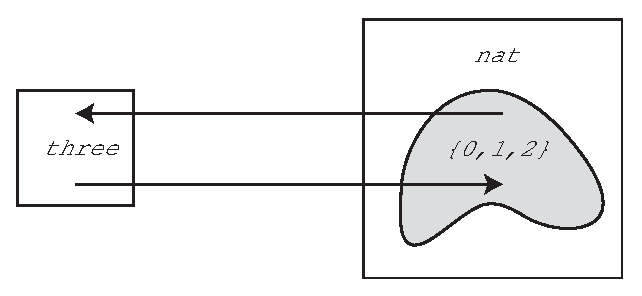
\includegraphics[scale=.8]{typedef}
\end{center}
Finally, \isacommand{typedef} asserts that \isa{Rep{\isacharunderscore}three} is
surjective on the subset \isa{three} and \isa{Abs{\isacharunderscore}three} and \isa{Rep{\isacharunderscore}three} are inverses of each other:
\begin{center}
\begin{tabular}{@ {}r@ {\qquad\qquad}l@ {}}
\isa{Rep{\isacharunderscore}three\ x\ {\isasymin}\ three} & (\isa{Rep{\isacharunderscore}three}) \\
\isa{Abs{\isacharunderscore}three\ {\isacharparenleft}Rep{\isacharunderscore}three\ x{\isacharparenright}\ {\isacharequal}\ x} & (\isa{Rep{\isacharunderscore}three{\isacharunderscore}inverse}) \\
\isa{y\ {\isasymin}\ three\ {\isasymLongrightarrow}\ Rep{\isacharunderscore}three\ {\isacharparenleft}Abs{\isacharunderscore}three\ y{\isacharparenright}\ {\isacharequal}\ y} & (\isa{Abs{\isacharunderscore}three{\isacharunderscore}inverse})
\end{tabular}
\end{center}
%
From this example it should be clear what \isacommand{typedef} does
in general given a name (here \isa{three}) and a set
(here \isa{{\isacharbraceleft}{\isadigit{0}}{\isacharcomma}\ {\isadigit{1}}{\isacharcomma}\ {\isadigit{2}}{\isacharbraceright}}).

Our next step is to define the basic functions expected on the new type.
Although this depends on the type at hand, the following strategy works well:
\begin{itemize}
\item define a small kernel of basic functions that can express all other
functions you anticipate.
\item define the kernel in terms of corresponding functions on the
representing type using \isa{Abs} and \isa{Rep} to convert between the
two levels.
\end{itemize}
In our example it suffices to give the three elements of type \isa{three}
names:%
\end{isamarkuptext}%
\isamarkupfalse%
\isacommand{constdefs}\isanewline
\ \ A{\isacharcolon}{\isacharcolon}\ three\isanewline
\ {\isachardoublequote}A\ {\isasymequiv}\ Abs{\isacharunderscore}three\ {\isadigit{0}}{\isachardoublequote}\isanewline
\ \ B{\isacharcolon}{\isacharcolon}\ three\isanewline
\ {\isachardoublequote}B\ {\isasymequiv}\ Abs{\isacharunderscore}three\ {\isadigit{1}}{\isachardoublequote}\isanewline
\ \ C\ {\isacharcolon}{\isacharcolon}\ three\isanewline
\ {\isachardoublequote}C\ {\isasymequiv}\ Abs{\isacharunderscore}three\ {\isadigit{2}}{\isachardoublequote}\isamarkuptrue%
%
\begin{isamarkuptext}%
So far, everything was easy. But it is clear that reasoning about \isa{three} will be hell if we have to go back to \isa{nat} every time. Thus our
aim must be to raise our level of abstraction by deriving enough theorems
about type \isa{three} to characterize it completely. And those theorems
should be phrased in terms of \isa{A}, \isa{B} and \isa{C}, not \isa{Abs{\isacharunderscore}three} and \isa{Rep{\isacharunderscore}three}. Because of the simplicity of the example,
we merely need to prove that \isa{A}, \isa{B} and \isa{C} are distinct
and that they exhaust the type.

In processing our \isacommand{typedef} declaration, 
Isabelle proves several helpful lemmas. The first two
express injectivity of \isa{Rep{\isacharunderscore}three} and \isa{Abs{\isacharunderscore}three}:
\begin{center}
\begin{tabular}{@ {}r@ {\qquad}l@ {}}
\isa{{\isacharparenleft}Rep{\isacharunderscore}three\ x\ {\isacharequal}\ Rep{\isacharunderscore}three\ y{\isacharparenright}\ {\isacharequal}\ {\isacharparenleft}x\ {\isacharequal}\ y{\isacharparenright}} & (\isa{Rep{\isacharunderscore}three{\isacharunderscore}inject}) \\
\begin{tabular}{@ {}l@ {}}
\isa{{\isasymlbrakk}x\ {\isasymin}\ three{\isacharsemicolon}\ y\ {\isasymin}\ three\ {\isasymrbrakk}} \\
\isa{{\isasymLongrightarrow}\ {\isacharparenleft}Abs{\isacharunderscore}three\ x\ {\isacharequal}\ Abs{\isacharunderscore}three\ y{\isacharparenright}\ {\isacharequal}\ {\isacharparenleft}x\ {\isacharequal}\ y{\isacharparenright}}
\end{tabular} & (\isa{Abs{\isacharunderscore}three{\isacharunderscore}inject}) \\
\end{tabular}
\end{center}
The following ones allow to replace some \isa{x{\isacharcolon}{\isacharcolon}three} by
\isa{Abs{\isacharunderscore}three{\isacharparenleft}y{\isacharcolon}{\isacharcolon}nat{\isacharparenright}}, and conversely \isa{y} by \isa{Rep{\isacharunderscore}three\ x}:
\begin{center}
\begin{tabular}{@ {}r@ {\qquad}l@ {}}
\isa{{\isasymlbrakk}y\ {\isasymin}\ three{\isacharsemicolon}\ {\isasymAnd}x{\isachardot}\ y\ {\isacharequal}\ Rep{\isacharunderscore}three\ x\ {\isasymLongrightarrow}\ P{\isasymrbrakk}\ {\isasymLongrightarrow}\ P} & (\isa{Rep{\isacharunderscore}three{\isacharunderscore}cases}) \\
\isa{{\isacharparenleft}{\isasymAnd}y{\isachardot}\ {\isasymlbrakk}x\ {\isacharequal}\ Abs{\isacharunderscore}three\ y{\isacharsemicolon}\ y\ {\isasymin}\ three{\isasymrbrakk}\ {\isasymLongrightarrow}\ P{\isacharparenright}\ {\isasymLongrightarrow}\ P} & (\isa{Abs{\isacharunderscore}three{\isacharunderscore}cases}) \\
\isa{{\isasymlbrakk}y\ {\isasymin}\ three{\isacharsemicolon}\ {\isasymAnd}x{\isachardot}\ P\ {\isacharparenleft}Rep{\isacharunderscore}three\ x{\isacharparenright}{\isasymrbrakk}\ {\isasymLongrightarrow}\ P\ y} & (\isa{Rep{\isacharunderscore}three{\isacharunderscore}induct}) \\
\isa{{\isacharparenleft}{\isasymAnd}y{\isachardot}\ y\ {\isasymin}\ three\ {\isasymLongrightarrow}\ P\ {\isacharparenleft}Abs{\isacharunderscore}three\ y{\isacharparenright}{\isacharparenright}\ {\isasymLongrightarrow}\ P\ x} & (\isa{Abs{\isacharunderscore}three{\isacharunderscore}induct}) \\
\end{tabular}
\end{center}
These theorems are proved for any type definition, with \isa{three}
replaced by the name of the type in question.

Distinctness of \isa{A}, \isa{B} and \isa{C} follows immediately
if we expand their definitions and rewrite with the injectivity
of \isa{Abs{\isacharunderscore}three}:%
\end{isamarkuptext}%
\isamarkupfalse%
\isacommand{lemma}\ {\isachardoublequote}A\ {\isasymnoteq}\ B\ {\isasymand}\ B\ {\isasymnoteq}\ A\ {\isasymand}\ A\ {\isasymnoteq}\ C\ {\isasymand}\ C\ {\isasymnoteq}\ A\ {\isasymand}\ B\ {\isasymnoteq}\ C\ {\isasymand}\ C\ {\isasymnoteq}\ B{\isachardoublequote}\isanewline
%
\isadelimproof
%
\endisadelimproof
%
\isatagproof
\isamarkupfalse%
\isacommand{by}{\isacharparenleft}simp\ add{\isacharcolon}\ Abs{\isacharunderscore}three{\isacharunderscore}inject\ A{\isacharunderscore}def\ B{\isacharunderscore}def\ C{\isacharunderscore}def\ three{\isacharunderscore}def{\isacharparenright}%
\endisatagproof
{\isafoldproof}%
%
\isadelimproof
%
\endisadelimproof
\isamarkuptrue%
%
\begin{isamarkuptext}%
\noindent
Of course we rely on the simplifier to solve goals like \isa{{\isadigit{0}}\ {\isasymnoteq}\ {\isadigit{1}}}.

The fact that \isa{A}, \isa{B} and \isa{C} exhaust type \isa{three} is
best phrased as a case distinction theorem: if you want to prove \isa{P\ x}
(where \isa{x} is of type \isa{three}) it suffices to prove \isa{P\ A},
\isa{P\ B} and \isa{P\ C}:%
\end{isamarkuptext}%
\isamarkupfalse%
\isacommand{lemma}\ three{\isacharunderscore}cases{\isacharcolon}\ {\isachardoublequote}{\isasymlbrakk}\ P\ A{\isacharsemicolon}\ P\ B{\isacharsemicolon}\ P\ C\ {\isasymrbrakk}\ {\isasymLongrightarrow}\ P\ x{\isachardoublequote}%
\isadelimproof
%
\endisadelimproof
%
\isatagproof
\isamarkuptrue%
%
\begin{isamarkuptxt}%
\noindent Again this follows easily from a pre-proved general theorem:%
\end{isamarkuptxt}%
\isamarkupfalse%
\isacommand{apply}{\isacharparenleft}induct{\isacharunderscore}tac\ x\ rule{\isacharcolon}\ Abs{\isacharunderscore}three{\isacharunderscore}induct{\isacharparenright}\isamarkuptrue%
%
\begin{isamarkuptxt}%
\begin{isabelle}%
\ {\isadigit{1}}{\isachardot}\ {\isasymAnd}y{\isachardot}\ {\isasymlbrakk}P\ A{\isacharsemicolon}\ P\ B{\isacharsemicolon}\ P\ C{\isacharsemicolon}\ y\ {\isasymin}\ three{\isasymrbrakk}\ {\isasymLongrightarrow}\ P\ {\isacharparenleft}Abs{\isacharunderscore}three\ y{\isacharparenright}%
\end{isabelle}
Simplification with \isa{three{\isacharunderscore}def} leads to the disjunction \isa{y\ {\isacharequal}\ {\isadigit{0}}\ {\isasymor}\ y\ {\isacharequal}\ {\isadigit{1}}\ {\isasymor}\ y\ {\isacharequal}\ {\isadigit{2}}} which \isa{auto} separates into three
subgoals, each of which is easily solved by simplification:%
\end{isamarkuptxt}%
\isamarkupfalse%
\isacommand{apply}{\isacharparenleft}auto\ simp\ add{\isacharcolon}\ three{\isacharunderscore}def\ A{\isacharunderscore}def\ B{\isacharunderscore}def\ C{\isacharunderscore}def{\isacharparenright}\isanewline
\isamarkupfalse%
\isacommand{done}%
\endisatagproof
{\isafoldproof}%
%
\isadelimproof
%
\endisadelimproof
\isamarkuptrue%
%
\begin{isamarkuptext}%
\noindent
This concludes the derivation of the characteristic theorems for
type \isa{three}.

The attentive reader has realized long ago that the
above lengthy definition can be collapsed into one line:%
\end{isamarkuptext}%
\isamarkupfalse%
\isacommand{datatype}\ better{\isacharunderscore}three\ {\isacharequal}\ A\ {\isacharbar}\ B\ {\isacharbar}\ C\isamarkuptrue%
%
\begin{isamarkuptext}%
\noindent
In fact, the \isacommand{datatype} command performs internally more or less
the same derivations as we did, which gives you some idea what life would be
like without \isacommand{datatype}.

Although \isa{three} could be defined in one line, we have chosen this
example to demonstrate \isacommand{typedef} because its simplicity makes the
key concepts particularly easy to grasp. If you would like to see a
non-trivial example that cannot be defined more directly, we recommend the
definition of \emph{finite multisets} in the Library~\cite{HOL-Library}.

Let us conclude by summarizing the above procedure for defining a new type.
Given some abstract axiomatic description $P$ of a type $ty$ in terms of a
set of functions $F$, this involves three steps:
\begin{enumerate}
\item Find an appropriate type $\tau$ and subset $A$ which has the desired
  properties $P$, and make a type definition based on this representation.
\item Define the required functions $F$ on $ty$ by lifting
analogous functions on the representation via $Abs_ty$ and $Rep_ty$.
\item Prove that $P$ holds for $ty$ by lifting $P$ from the representation.
\end{enumerate}
You can now forget about the representation and work solely in terms of the
abstract functions $F$ and properties $P$.%
\index{typedecl@\isacommand {typedef} (command)|)}%
\index{types!defining|)}%
\end{isamarkuptext}%
%
\isadelimtheory
%
\endisadelimtheory
%
\isatagtheory
%
\endisatagtheory
{\isafoldtheory}%
%
\isadelimtheory
%
\endisadelimtheory
\end{isabellebody}%
%%% Local Variables:
%%% mode: latex
%%% TeX-master: "root"
%%% End:
    %%%Section "Introducing New Types"
